\documentclass[11pt]{article}
\ifdefined\pdfinfoomitdate\pdfinfoomitdate=1\fi
\ifdefined\pdftrailerid\pdftrailerid{}\fi
\ifdefined\pdfsuppressptexinfo\pdfsuppressptexinfo=15\fi
\usepackage[T1]{fontenc}
\usepackage{lmodern}
\input{glyphtounicode}
\pdfglyphtounicode{braceleftbigg}{007B}
\pdfglyphtounicode{bracerightbigg}{007D}
\pdfglyphtounicode{bracketleftbig}{005B}
\pdfglyphtounicode{bracketleftbigg}{005B}
\pdfglyphtounicode{bracketleftbt}{23A3}
\pdfglyphtounicode{bracketlefttp}{23A1}
\pdfglyphtounicode{bracketrightbig}{005D}
\pdfglyphtounicode{bracketrightbigg}{005D}
\pdfglyphtounicode{bracketrightbt}{23A6}
\pdfglyphtounicode{bracketrighttp}{23A4}
\pdfglyphtounicode{hatwide}{0302}
\pdfglyphtounicode{hatwider}{0302}
\pdfglyphtounicode{integraldisplay}{222B}
\pdfglyphtounicode{integraltext}{222B}
\pdfglyphtounicode{mapsto}{007C}
\pdfglyphtounicode{parenleftBig}{0028}
\pdfglyphtounicode{parenleftBigg}{0028}
\pdfglyphtounicode{parenleftbig}{0028}
\pdfglyphtounicode{parenleftbigg}{0028}
\pdfglyphtounicode{parenleftbt}{239D}
\pdfglyphtounicode{parenlefttp}{239B}
\pdfglyphtounicode{parenrightBig}{0029}
\pdfglyphtounicode{parenrightBigg}{0029}
\pdfglyphtounicode{parenrightbig}{0029}
\pdfglyphtounicode{parenrightbigg}{0029}
\pdfglyphtounicode{parenrightbt}{23A0}
\pdfglyphtounicode{parenrighttp}{239E}
\pdfglyphtounicode{productdisplay}{220F}
\pdfglyphtounicode{producttext}{220F}
\pdfglyphtounicode{radicalBig}{221A}
\pdfglyphtounicode{radicalBigg}{221A}
\pdfglyphtounicode{radicalbig}{221A}
\pdfglyphtounicode{summationdisplay}{2211}
\pdfglyphtounicode{summationtext}{2211}
\pdfglyphtounicode{tildewide}{0303}
\pdfglyphtounicode{vextenddouble}{2225}
\pdfglyphtounicode{vextendsingle}{007C}
\pdfgentounicode=1

\usepackage[margin=1in]{geometry}
\usepackage{amsmath,amssymb,amsthm,mathtools}
\usepackage{microtype}
\usepackage{needspace}
\usepackage{enumitem}
\usepackage{booktabs}
\usepackage{tikz}
\usetikzlibrary{arrows.meta,positioning}
\usepackage[numbers,sort&compress]{natbib}
\usepackage[colorlinks=true,linkcolor=blue!55!black,citecolor=blue!55!black,urlcolor=blue!55!black]{hyperref}
\usepackage[nameinlink,capitalise,noabbrev]{cleveref}
\hypersetup{pdftitle={GOE bulk universality for fixed-degree random regular graphs},pdfauthor={OpenAI}}
\newtheorem{theorem}{Theorem}[section]
\newtheorem{proposition}[theorem]{Proposition}
\newtheorem{lemma}[theorem]{Lemma}
\newtheorem{corollary}[theorem]{Corollary}
\theoremstyle{definition}
\newtheorem{definition}[theorem]{Definition}
\theoremstyle{remark}
\newtheorem{remark}[theorem]{Remark}
\AddToHook{env/theorem/before}{\Needspace{5\baselineskip}}
\AddToHook{env/proposition/before}{\Needspace{5\baselineskip}}
\AddToHook{env/lemma/before}{\Needspace{5\baselineskip}}
\numberwithin{equation}{section}
\newcommand{\R}{\mathbb R}
\newcommand{\C}{\mathbb C}
\newcommand{\N}{\mathbb N}
\newcommand{\PP}{\mathbb P}
\newcommand{\EE}{\mathbb E}
\newcommand{\Id}{I}
\newcommand{\HS}{\mathrm{HS}}
\newcommand{\TV}{\mathrm{TV}}
\newcommand{\dd}{\,\mathrm d}
\newcommand{\eps}{\varepsilon}
\newcommand{\ip}[2]{\langle #1,#2\rangle}
\DeclareMathOperator{\Tr}{Tr}
\DeclareMathOperator{\Var}{Var}
\DeclareMathOperator{\Cov}{Cov}
\DeclareMathOperator{\diag}{diag}
\DeclareMathOperator{\rank}{rank}
\DeclareMathOperator{\spanop}{span}
\DeclareMathOperator{\supp}{supp}
\DeclareMathOperator{\dist}{dist}
\DeclareMathOperator{\GOE}{GOE}
\DeclareMathOperator{\PV}{PV}
\DeclareMathOperator{\Ent}{Ent}
\DeclareMathOperator{\Law}{Law}
\newcommand{\op}{\mathrm{op}}
\setlist[enumerate]{itemsep=3pt,topsep=5pt}
\setlist[itemize]{itemsep=3pt,topsep=5pt}
\setlength{\emergencystretch}{2em}
\title{GOE bulk universality for fixed-degree random regular graphs}
\author{OpenAI}
\date{September 23, 2026}
\begin{document}
\maketitle
\begin{abstract}
We prove the fixed-degree bulk-universality conjecture for random regular graphs. For every fixed integer \(d\ge3\) and every fixed energy in the open Kesten--McKay bulk, the unfolded eigenvalue point process of the adjacency matrix of a uniform simple labelled \(d\)-regular graph converges to the GOE bulk process. The convergence holds along all admissible graph sizes, without additional conditioning.
\end{abstract}
\section{Introduction}\label{sec:introduction}

A random regular graph is sparse even when its order tends to infinity:
each row of its adjacency matrix has exactly \(d\) nonzero entries.
Nevertheless, its bulk eigenvalues are expected to exhibit the local
statistics of a real symmetric Gaussian matrix.
We prove this prediction for every fixed degree \(d\ge3\), at each fixed
energy in the interior of the limiting spectrum.

\subsection{Main result}

For an admissible integer \(n\), let \(G_{n,d}\) be uniform among the
simple labelled \(d\)-regular graphs on \(\{1,\ldots,n\}\).
Here admissible means that this set is nonempty.
Let \(A_{n,d}\) be its unweighted adjacency matrix, with eigenvalues
\(\lambda_1,\ldots,\lambda_n\), counted with multiplicity.
No conditioning on connectedness, bipartiteness, or another graph
property is imposed.

The limiting density is the Kesten--McKay density
\[
 \rho_d(t)=\frac{d\sqrt{4(d-1)-t^2}}{2\pi(d^2-t^2)}
 \qquad \bigl(|t|<2\sqrt{d-1}\bigr).
\]
For a fixed energy \(E\) in this interval, define the unfolded
point measure
\[
 \Xi_{n,d,E}=\sum_{i=1}^n
       \delta_{\,n\rho_d(E)(\lambda_i-E)}.
\]
For comparison, let \(H_n\) be a normalized GOE matrix: its entries on
and above the diagonal are independent centered Gaussians, with
variance \(1/n\) off the diagonal and \(2/n\) on the diagonal.
If \(\mu_1,\ldots,\mu_n\) are its eigenvalues, put
\[
 \Xi_n^{\mathrm{GOE}}
       =\sum_{i=1}^n\delta_{(n/\pi)\mu_i}.
\]

\newpage
\begin{theorem}\label{thm:main}
For every fixed integer \(d\ge3\), every fixed
\(E\in(-2\sqrt{d-1},2\sqrt{d-1})\), and every nonnegative continuous
compactly supported \(h:\R\to\R\),
\[
 \left|
 \EE\exp\!\left(-\int h\dd\Xi_{n,d,E}\right)
 -
 \EE\exp\!\left(-\int h\dd\Xi_n^{\mathrm{GOE}}\right)
 \right|\longrightarrow0
\]
as \(n\to\infty\) through all admissible sizes.
\end{theorem}

The GOE reference point measures converge in law for the vague
topology \cite{ValkoVirag}.
Thus Theorem~\ref{thm:main} identifies the full local point-process
limit, not only its one-point density or an energy-averaged statistic.
It proves the fixed-degree bulk-universality conjecture stated in
\cite[Conjecture 2.11]{BourgadeHuang}, in a fixed-energy
Laplace-functional formulation.

\subsection{Background and significance}

The density above originates in the spectral measure of the regular
tree and the limiting spectrum of random regular graphs
\cite{Kesten,McKay}.
It describes eigenvalue counts on macroscopic intervals, but does not
determine the spacings between consecutive eigenvalues.
Jakobson, Miller, Rivin, and Rudnick
\cite[Sections~1 and~5]{JakobsonEtAl} formulated the GOE prediction
for fixed-degree regular graphs and gave numerical evidence for it.
Their empirical nearest-neighbor spacing formulation precedes the
fixed-energy point-process formulation studied here.
The prediction is particularly striking at fixed degree: local tree
geometry persists, whereas the proposed eigenvalue statistics agree
with those of a dense Gaussian matrix.

The development of local laws separated spectral control from the
identification of microscopic statistics. Bauerschmidt, Knowles, and
Yau \cite{BauerschmidtKnowlesYauLocal} established a local semicircle
law for growing degrees using local resampling. Bauerschmidt, Huang,
Knowles, and Yau \cite[Theorems 1.1 and 1.2]{BauerschmidtEtAl}
proved bulk gap universality and energy-averaged correlation
universality in a polynomial degree range. More recently, Bourgade
and Huang \cite[Proposition 2.10]{BourgadeHuang} obtained fixed-energy
point-process universality for
\((\log n)^{24}\ll d\le n^{1/2}\) by loop equations, and stated the
remaining fixed-degree problem in their Conjecture 2.11.

For fixed degree the local reference law is Kesten--McKay.
Bauerschmidt, Huang, and Yau \cite{BauerschmidtHuangYauLocal}
established the local law and delocalization for sufficiently large
fixed degrees. Huang and Yau \cite{HuangYau} subsequently proved
rigidity, complete delocalization, and local resolvent estimates for
every fixed \(d\ge3\). Their estimates supply the spectral input for
this paper. They control smoothed eigenvalue counts and typical tree
neighborhoods, while the conclusion sought here concerns unsmoothed
statistics at one fixed energy on the scale of an individual spacing.

For every fixed \(d\ge3\), Huang, McKenzie, and Yau
\cite[Theorems~1.1 and~1.2]{HuangMcKenzieYau}
proved optimal eigenvalue rigidity, up to subpolynomial factors,
and GOE edge universality.
Their edge result identifies the joint fluctuations of any fixed
number of extreme nontrivial eigenvalues at either spectral edge.

Eigenvector Gaussianity provides the link we need from spectral control
to microscopic bulk statistics.
The Gaussian-wave model on a regular tree appears in
\cite{ElonEigenvectors,CsokaEtAl}.
Backhausz and Szegedy \cite[Theorems 2.1 and 2.2]{BackhauszSzegedy}
proved qualitative Gaussian-wave limits for almost eigenvectors of
random regular graphs, allowing a variance factor between zero and
one in the weak limit. Their argument uses entropy inequalities for
local observations; the underlying colored-star counting framework
was developed in \cite{BackhauszSzegedyTrees} and further studied in
\cite{BackhauszBordenaveSzegedy}. Recent developments include
variance-one Gaussian waves for spectral-edge eigenvectors
\cite{HeHuangYauWaves} and an extension of the entropy framework to
graphs of finite cone type \cite{DemboMcKenzie}.
Our argument develops this entropy method into a different input:
polynomially accurate, variance-one joint moments at sampled graph
edges. The estimates hold conditional on each graph in an event of
probability tending to one, uniformly over finitely many chosen bulk
eigenvectors. Weak convergence alone does not provide
these high-moment estimates. The proof below supplies them through
a strict tensor estimate and a quantitative Hermite expansion.

Reversible edge switches are also established tools in local laws
and universality; see \cite[Section 3]{BauerschmidtEtAl} and
\cite[Section 7.2]{BauerschmidtHuangYauLocal}.
We use Gaussian endpoint marks to extend the discrete symmetry to
an orthogonal action on an exact microscopic limiting law. Increasing
the number of sampled edge pairs within that limit then inserts a Gaussian
matrix perturbation. The last step uses the local relaxation of
Dyson's matrix evolution \cite{DysonBrownian,LandonYau}, in the
fixed-energy form proved by Landon, Sosoe, and Yau
\cite{LandonSosoeYau}. To obtain the full point-process conclusion
from fixed-order correlations, we also give a compact-count bound
using the Gaussian superposition and decimation identity of
Forrester and Rains \cite{ForresterRains}.

\subsection{Proof strategy}

We first work in the coordinates \(x_i=n(\lambda_i-E)\), before the
last density factor \(\rho_d(E)\) is applied.
For a real eigenvector normalized to have squared norm \(n\), sampling
its values at the two ends of a uniform oriented edge produces a pair
of random real numbers. We call each sampled edge and its two endpoint
coordinates a channel.
The first part of the proof shows that, for any fixed number of
eigenvectors near \(E\), every fixed joint moment of these sampled
values is polynomially close to the corresponding Gaussian moment,
with probability tending to one over the graph.
The comparison consists of centered, unit-variance Gaussian pairs,
independent across the eigenvectors, with covariance \(E/d\) within each pair.

The following steps then identify every subsequential microscopic
point-process limit.

\begin{enumerate}
\item \emph{Quantitative Gaussian marks.}
Section~\ref{sec:entropy} proves the endpoint moment statement.
A colored-star counting inequality becomes an entropy inequality after
the eigenvectors are smoothed by a Gaussian field.
The tree logarithmic potential evaluates the entropy cost.
A strict tensor inequality turns the resulting entropy deficit into
Gaussian moment matching by induction over Hermite degree.

\item \emph{Microscopic limits with controlled tails.}
Section~\ref{sec:limits} uses a two-edge switch and the moment statement
to control resolvents at large fixed microscopic heights.
It then extracts the point process together with its Gaussian endpoint
marks. The limiting resolvent has a symmetric principal-value
representation, and the point counts have a power-saving discrepancy
from constant density.

\item \emph{Continuous switching and Gaussian insertion.}
Section~\ref{sec:switching} combines the discrete switch symmetry with
orthogonal invariance of the Gaussian marks.
This produces exact continuous switching identities for the
microscopic limiting law.
After two controlled truncations, many weak switches give finite
diagonal matrices with additive GOE noise whose eigenvalue point
processes converge to that same limiting law.

\item \emph{Identification at one energy.}
Section~\ref{sec:dbm} verifies the hypotheses of fixed-energy Dyson
Brownian motion universality for these diagonal matrices.
An exact adjustment of the free-convolution density matches the
normalizations of the two ensembles.
A uniform exponential bound for compact GOE counts and finite
inclusion-exclusion then upgrade correlation comparisons to the
Laplace functionals in Theorem~\ref{thm:main}.
\end{enumerate}

Two parts of this argument are useful beyond the final identification.
The entropy calculation gives Gaussian moment approximation with
polynomially small errors on common graph events of probability tending
to one, including graph-dependent choices of eigenvectors; its strictness
is a finite-dimensional tensor fact tied
to the open bulk and to \(d\ge3\).
The continuous switching argument converts a discrete finite-rank
symmetry into Gaussian perturbations of an exact limiting marked
process. The latter mechanism requires only fixed-dimensional
Gaussian information before the limit.

The passage from finitely many Gaussian marks to many weak switches
takes place after the graph-size limit. We first let \(n\to\infty\)
with fixed numbers of sampled edges and fixed spectral windows, then
control the tails to construct the principal-value marked law in
Section~\ref{sec:limits}. Its switching identities are exact for every
fixed number of channels. Only within this law do we let the channel
number \(k=2r\) tend to infinity, with the two spectral cutoffs prescribed
in Section~\ref{sec:switching}. Finally we increase the order of the
inclusion-exclusion brackets in Section~\ref{sec:dbm}. Thus the
finite-graph argument requires Gaussian approximation only in fixed
dimensions and at fixed moment orders.

\section{Spectral input and tree identities}\label{sec:preliminaries}

Throughout the proof, \(d\ge3\) and \(|E|<2\sqrt{d-1}\) are fixed.
All constants may depend on these two parameters.
This section records the spectral information used below and the tree
identities that determine the covariance of the eigenvector entries.
The spectral estimates are established results; the subsequent entropy
and switching arguments are proved in this paper.

\subsection{Conventions and microscopic coordinates}

Let
\[
 \rho_d(t)=
 \frac{d\sqrt{4(d-1)-t^2}}{2\pi(d^2-t^2)}
 \mathbf 1_{\{|t|<2\sqrt{d-1}\}},
 \qquad
 m_d(\zeta)=\int_{\R}\frac{\rho_d(t)}{t-\zeta}\dd t
 \quad(\Im\zeta>0).
\]
Set
\[
 \rho=\rho_d(E),\qquad p=\frac Ed,\qquad
 a=\frac{d}{d-1}(1-p^2),\qquad
 m_*=m_d(E+\mathrm i0)=m_{\rm r}+\mathrm i\pi\rho.
\]
In particular, \(\rho>0\), \(a>0\), and \(|p|<1\).
For the adjacency eigenvalues and a graph-determined real orthogonal
eigenbasis, use the normalization
\[
 Au_i=\lambda_i u_i,\qquad
 \langle u_i,u_j\rangle=n\delta_{ij}.
\]
An arbitrary measurable choice inside each eigenspace suffices.
Define
\begin{equation}\label{eq:micro-coordinates}
 x_i=n(\lambda_i-E),\qquad
 \nu_n=\sum_{i=1}^n\delta_{x_i},\qquad
 m_n(z)=\sum_{i=1}^n\frac1{x_i-z}
       =\frac1n\Tr R_n(z),
 \quad
 R_n(z)=(A-E-z/n)^{-1}.
\end{equation}
The remaining density factor for unfolding is \(\rho\); the final
point coordinates are obtained by multiplying the \(x_i\) by \(\rho\).
We write \(\C_+=\{z\in\C:\Im z>0\}\) for the upper half-plane.

For \(k\ge1\), let
\begin{equation}\label{eq:channel-matrices}
 J_k=\begin{pmatrix}0&I_k\\ I_k&0\end{pmatrix},
 \qquad C_k=I_{2k}+pJ_k,\qquad
 K_k(m)=mC_k+d^{-1}J_k.
\end{equation}
The order of the \(2k\) coordinates will always be the starting endpoints
of \(k\) oriented edges, followed by their ending endpoints.
The matrix \(C_k\) is positive definite.

Unsubscripted finite-dimensional matrix norms are operator norms;
\(\|\cdot\|_{\HS}\) denotes the Hilbert--Schmidt norm.
The imaginary part of a matrix is its Hermitian imaginary part.
For the complex symmetric matrices occurring here it also agrees with
entrywise imaginary part.
All tensor norms are induced by the stated Euclidean inner products.
The notation \(n^{o(1)}\), when used on high-probability events, denotes a
deterministic subpolynomial upper bound.
We write \(O_{\PP}(b_r)\) for a random quantity whose ratio to \(b_r\) is
bounded in probability; \(o_{\PP}(b_r)\) means that the ratio tends
to zero in probability.

\subsection{The simple regular-graph model}

We use the classical pairing model for regular graphs
\cite{BollobasPairing}. The special counting facts needed here have
the following direct proof.

\begin{lemma}\label{lem:model}
In the configuration model with \(d\) stubs at each of \(n\) labelled
vertices, conditioning the matching to give a simple graph produces the
uniform simple labelled \(d\)-regular graph. Moreover,
\[
 \PP(\text{the matching gives a simple graph})
       \longrightarrow \exp\!\left(-\frac{d^2-1}{4}\right)>0
\]
along all admissible sizes.
In the simple model, a specified vertex belongs to a triangle with
probability \(O(n^{-1})\).
For any fixed \(k\), independently sampled uniform oriented edges have
distinct endpoints and induce exactly a matching with probability
\(1-O_k(n^{-1})\).
\end{lemma}

\begin{proof}
Every simple graph has the same number \((d!)^n\) of stub realizations,
which proves the conditional uniformity.
A prescribed loop is one pair of stubs at a vertex. A prescribed
double edge is an unordered pair of pairs between two distinct vertices,
using distinct stubs. Let \(Z\) count all occurring prescribed defects
of these two kinds.
The expected counts tend to
\[
 \frac{d-1}{2}\quad\hbox{and}\quad\frac{(d-1)^2}{4},
\]
respectively.
Indeed, a prescribed family of \(e\) disjoint pairs occurs with
probability
\[
 \frac{1}{(nd-1)(nd-3)\cdots(nd-2e+1)}
       \sim(nd)^{-e}
\]
for fixed \(e\).

For each fixed \(j\), ordered \(j\)-tuples of defects on disjoint vertex
sets give the leading contribution to \(\EE(Z)_j\).
Compatible overlapping tuples contribute \(o(1)\).
To see this, regard their prescribed pairs as a multigraph with \(v\)
vertices and \(e\) edges. Every vertex has degree at least two. A
connected component all of whose degrees equal two can only be a
single prescribed loop or a single prescribed double edge.
Thus a genuinely overlapping component has \(v<e\). There are
\(O(n^v)\) choices and each has probability \(O(n^{-e})\).
There are only finitely many overlap patterns for fixed \(d,j\).
Consequently
\[
 \EE(Z)_j\longrightarrow
 \left(\frac{d-1}{2}+\frac{(d-1)^2}{4}\right)^j.
\]
The finite inclusion-exclusion bounds for \(\PP(Z=0)\), followed by
increasing their order, give the asserted limit. Absence of these
defects is exactly simplicity.

For a triangle through a fixed vertex, summing over the other two
vertices and their stub choices gives
\(O(n^2)\,O(n^{-3})=O(n^{-1})\) in the matching model.
Conditioning on simplicity changes this bound by a bounded factor.
Finally, in any simple \(d\)-regular graph a uniform endpoint is a
uniform vertex. Each previously chosen endpoint has only \(O_d(1)\)
vertices equal or adjacent to it. A union bound over the fixed number
of sampled endpoints proves the last assertion.
\end{proof}

\subsection{The imported spectral estimates}

Put
\[
 S=\exp(\sqrt{\log n}).
\]
The following deliberately weak formulation is sufficient for our
argument.

\begin{proposition}[Spectral input]\label{prop:spectral-input}
There are constants \(c_0,c_1>0\), \(B<\infty\), and a fixed open interval
\(I_E\) containing \(E\), with closure contained in
\((-2\sqrt{d-1},2\sqrt{d-1})\), such that the following hold with probability
tending to one.

\begin{enumerate}
\item After omitting the eigenvalue associated with the constant vector,
the ordered eigenvalues are within \(n^{-c_0}\) of their
Kesten--McKay classical locations. In the normalization above, every
eigenvector entry is bounded by a deterministic \(n^{o(1)}\).
\item Uniformly for \(\Re\zeta\in I_E\) and \(S/n\le\Im\zeta\le1\),
\[
 \left|\frac1n\Tr(A-\zeta)^{-1}-m_d(\zeta)\right|
 \le(\log n)^B\bigl(n^{-c_1}+(n\Im\zeta)^{-c_1}\bigr).
\]
Except at at most \(n^{1-c_1}\) centers, the resolvent entries on a
center and its \(d\) neighbors satisfy the same error bound relative
to the corresponding infinite \(d\)-regular tree entries.
\end{enumerate}
These conclusions hold along all admissible \(n\). In particular,
\[
 \#\{i:|x_i|\le S^2\}=O(S^2)
\]
on an event of probability tending to one.
\end{proposition}

\begin{proof}
We use the fixed-degree results of Huang and Yau
\cite[Theorems 1.2, 1.4, and 4.2]{HuangYau}, in the precise version
arXiv:2102.00963v3.
Their matrix is \(A/\sqrt{d-1}\); hence their bulk coordinate is
\(E/\sqrt{d-1}\in(-2,2)\).
Rescaling the spectral parameter and the resolvent by this fixed factor
gives our normalization.

For clarity, the relevant error and geometry can be checked directly
in their Definition 4.1 and Equations (4.6)--(4.7).
Choose fixed parameters
\[
 0<c<1,\qquad a_{\mathrm{HY}}\ge12,\qquad
 b_{\mathrm{HY}}\ge25a_{\mathrm{HY}},\qquad
 0<\mathfrak r<c/32,
\]
and neighborhood radius
\(r_{\mathrm{HY}}=\mathfrak r\log_{d-1}n\), rounded to an integer.
Their Definition 1.1 and Proposition 2.1 give a tree-like event with
probability tending to one, on which all but a polynomially small
fraction of vertices have a tree neighborhood of radius
\((c/4)\log_{d-1}n\).
This is more than enough to contain every neighborhood needed for the
resolvent approximation between two vertices of the same star.
The tree extension with the semicircle weight in their Equation (2.12)
is then the ordinary regular-tree Green function.

In a fixed bulk interval, their error is bounded by a logarithmic
factor times
\[
 (d-1)^{-r_{\mathrm{HY}}}
 +(n\Im\zeta)^{-1/2}
 +(n\Im\zeta)^{-2/3}.
\]
The factor \(S\) dominates every fixed power of \(\log n\).
After decreasing \(c_1\) and increasing \(B\), this gives the stated
bounds and exceptional-set size. The same source provides polynomial
rigidity and polylogarithmic complete delocalization.
Its model and the quoted statements have no even-size restriction.

For the final assertion, apply the trace estimate at
\(\zeta=E+\mathrm iS^2/n\). Each eigenvalue with
\(|\lambda_i-E|\le S^2/n\) contributes at least
\(n/(2S^2)\) to \(\Im(\lambda_i-\zeta)^{-1}\).
The normalized imaginary trace is bounded, so the count is \(O(S^2)\).
\end{proof}

\begin{remark}
The estimates in Proposition~\ref{prop:spectral-input} are statements
about events in the unconditioned simple-graph ensemble. We never
condition the conclusion of Theorem~\ref{thm:main} on connectedness,
nonbipartiteness, or a tree-neighborhood property.
The bounded Laplace observables are unaffected in the limit by
discarding events of vanishing probability.
\end{remark}

\subsection{Covariance and logarithmic potential on the tree}

The covariance below is the Gaussian-wave covariance on the regular
tree; see \cite{ElonEigenvectors,CsokaEtAl}. We derive it together with
the logarithmic potential, so that the entropy normalization is explicit.

\begin{lemma}\label{lem:tree-identities}
Let \(q(\zeta)\) be the solution of
\[
 \zeta=q^{-1}+(d-1)q
\]
which tends to zero at infinity in the upper half-plane.
Then
\[
 -m_d(\zeta)=\frac1{\zeta-dq(\zeta)}.
\]
The regular-tree resolvent has diagonal entry \(m_d(\zeta)\) and
adjacent entry \((1+\zeta m_d(\zeta))/d\).
At \(\zeta=E+\mathrm i\eta\), its imaginary-part matrix on a star,
divided by \(\pi\rho\), tends at a polynomial rate in \(\eta\) to the
covariance matrix with variances one, center-neighbor covariance \(p\),
and distinct-neighbor covariance
\[
 \frac{E^2-d}{d(d-1)}.
\]
Furthermore,
\[
 k_0=\frac{1+Em_*}{d}
 \quad\Longrightarrow\quad
 k_0^2-k_0-m_*^2=0.
\]
For \(U(E)=\int\log|t-E|\rho_d(t)\dd t\),
\begin{equation}\label{eq:tree-potential}
 -U(E)=-\frac12\log d+\frac{d-1}{2}\log a
                       -\frac d4\log(1-p^2).
\end{equation}
Replacing \(E\) by \(E+\mathrm i\eta\) in the logarithmic potential
changes its real part by \(O(\eta)\).
\end{lemma}

\begin{proof}
A Schur complement at the root of a forward tree gives
\(q=(\zeta-(d-1)q)^{-1}\) in the convention \((\zeta-A)^{-1}\).
Attaching \(d\) forward branches yields the displayed formula for
\(-m_d\). The boundary value
\(\pi^{-1}\Im m_d(t+\mathrm i0)\) is the Kesten--McKay density above;
the branch has the required mass at infinity and no additional pole.

The resolvent equation at the center and symmetry among its neighbors
give the adjacent entry. Applying the same equation to a neighbor
column gives, for the common distinct-neighbor entry \(g_2\),
\[
 m_d(\zeta)+(d-1)g_2
       =\zeta\,\frac{1+\zeta m_d(\zeta)}d.
\]
Taking boundary imaginary parts proves the covariance formulas.
The tree formula is analytic across each side of a sufficiently small
bulk neighborhood, so these limits have a polynomial rate.
Substituting its boundary value into \(k_0=(1+Em_*)/d\) gives the
quadratic identity.

To compute the potential, integrate its analytic derivative
\(-m_d(\zeta)=q/(1-q^2)\) after changing from \(\zeta\) to \(q\).
Matching at infinity gives
\[
 \Re\int\log(\zeta-t)\rho_d(t)\dd t
       =-\log|q|-\frac{d-2}{2}\log|1-q^2|.
\]
At the bulk boundary,
\[
 |q|=(d-1)^{-1/2},\qquad
 |1-q^2|=\frac{\sqrt{d^2-E^2}}{d-1}.
\]
These identities give \eqref{eq:tree-potential} after substituting
\(a=d(1-p^2)/(d-1)\).
The boundary logarithmic integral exists because \(\rho_d\) is bounded
near \(E\). Finally,
\[
 \int \left(\log|t-E-\mathrm i\eta|-\log|t-E|\right)\rho_d(t)\dd t
 =\frac12\int\log\!\left(1+\frac{\eta^2}{(t-E)^2}\right)\rho_d(t)\dd t
 =O(\eta),
\]
by boundedness of the density near \(E\), the substitution
\(t-E=\eta u\), and the integrable tail of \(\log(1+u^{-2})\).
\end{proof}

\section{Gaussian moments at sampled edges}\label{sec:entropy}

We use the spectral estimates of Proposition~\ref{prop:spectral-input}
to identify the empirical distribution of finitely many eigenvector
coordinates at an edge. The estimate must be quantitative: a fixed
moment will later be summed over a subpolynomial number of eigenindices.
We develop the entropy framework of \citet{BackhauszSzegedy}
quantitatively to obtain the conditional moment accuracy required here.

\begin{proposition}[Uniform endpoint moments]\label{prop:edge-moments}
Fix positive integers \(k,\ell\) and a nonnegative integer \(q\).
There are constants \(c,C>0\) and events of graphs of probability tending
to one with the following property. Choose distinct indices
\(i(1),\ldots,i(\ell)\) satisfying \(|x_{i(j)}|\le S^2\), by any rule
depending only on the graph. Independently sample \(k\) uniform oriented
edges \((v_\alpha,v'_\alpha)\), conditionally on the graph, and set
\[
 b_j=\bigl(u_{i(j)}(v_1),\ldots,u_{i(j)}(v_k),
           u_{i(j)}(v'_1),\ldots,u_{i(j)}(v'_k)\bigr)^\top .
\]
For every coordinate monomial \(P\) of total degree at most \(q\),
\[
 \left|\EE\bigl[P(b_1,\ldots,b_\ell)\mid A\bigr]
       -\EE P(Z_1,\ldots,Z_\ell)\right|\le Cn^{-c},
 \qquad Z_1,\ldots,Z_\ell\ \text{independent }N(0,C_k).
\]
The constants and graph events are uniform over the indicated choices
of eigenindices. They may depend on \(d,E,k,\ell,q\); no assertion is
made for dimensions or moment orders growing with \(n\).
\end{proposition}

We first prove the assertion for one sampled edge. Write
\[
 V(v)=\bigl(u_{i(1)}(v),\ldots,u_{i(\ell)}(v)\bigr)\in\R^\ell.
\]
A star observation consists of the value at a uniform vertex followed
by its \(d\) neighbor values in uniform random order. An edge observation
uses a uniform oriented edge. Throughout this section the graph is
conditioned on, and randomness in an observation includes its location.
Write \(H\) for discrete entropy and \(\mathcal H\) for differential
entropy, both with natural logarithms. Positive polynomial error
exponents may decrease from one occurrence to the next.

The proof passes from colored-label counts to an entropy inequality
for Gaussian-smoothed stars and edges. We remove the nearly
deterministic eigenvector relation, then use tensor coercivity to turn
the resulting entropy bound into Gaussian moment estimates.

\subsection{Counting colored stars}

We begin with a counting statement independent of eigenvectors.
For a labeling of the vertices by an alphabet of size \(M\), let \(T\)
be the probability distribution of the ordered star observation,
symmetrized over all permutations of the neighbor positions. Let \(Q\)
be the oriented edge distribution.
The counting argument follows the colored-star configuration-model
framework of \citet[Section~4]{BackhauszSzegedyTrees}; see also the
asymptotic expected-coloring formula of
\citet[Theorem~2.3]{BackhauszBordenaveSzegedy}.
We retain explicit errors for an alphabet growing with \(n\).

\begin{lemma}[Uniform type count]\label{ent:type-count}
Suppose \(M=M_n\) and, for some fixed \(\kappa>0\),
\(M^{d+1}\log n\le n^{1-\kappa}\).
With probability tending to one, simultaneously for every pair of
histograms \(T,Q\), the number of vertex labelings with these histograms
is at most
\begin{equation}\label{eq:ent-type-count}
 \exp\left\{nH(T)-\frac{nd}{2}H(Q)+O(n^{1-c})\right\},
\end{equation}
where \(c>0\) and the error constant depend only on \(d,\kappa\).
\end{lemma}

\begin{proof}
Work first in the configuration model, with an ordering of the \(d\)
half-edges at each vertex. Prescribe the vertex labels and the ordered
list of desired neighbor labels at every vertex. For a fixed ordered
tuple type \(T_0\), there are at most \(\exp(nH(T_0))\) such arrays, by
the multinomial bound.

Let \(m_{jk}=ndQ_{jk}\) be the number of half-edges whose vertex has
color \(j\) and whose prescribed neighbor has color \(k\).
Compatibility requires \(m_{jk}=m_{kj}\), and \(m_{jj}\) must be even.
The probability that a uniform matching respects all these prescriptions is
\[
 \frac{\displaystyle\prod_{j<k}m_{jk}!
                    \prod_j(m_{jj}-1)!!}{(nd-1)!!},
\]
with zero-size factors omitted. Stirling's bounds give its logarithm as
\[
 -\frac{nd}{2}H(Q)+O(M^2\log n).
\]
Thus the expected number of labelings of ordered type \(T_0\) has the
claimed exponential bound with \(H(T_0)\) in place of \(H(T)\).

Symmetrization increases entropy, so \(H(T_0)\le H(T)\); it leaves \(Q\)
unchanged. There are at most
\(\exp(O(M^{d+1}\log n))\) possible ordered tuple types. Summing over
those with a given symmetrization therefore changes only the sublinear
error. Markov's inequality, followed by a union bound over all types,
gives \eqref{eq:ent-type-count} with a slightly larger sublinear
allowance. The simplicity probability is bounded away from zero by
Lemma~\ref{lem:model}, so the statement transfers to uniform simple
graphs. The symmetrized histograms no longer depend on the half-edge
ordering.
\end{proof}

\subsection{A quantitative differential-entropy inequality}

Choose small fixed parameters \(\gamma,\alpha>0\) satisfying
\begin{equation}\label{eq:ent-parameters}
 2\ell(d+1)\gamma<1,\qquad
 4\ell\gamma+\alpha<\frac14,\qquad
 0<\alpha<\gamma,
\end{equation}
and take \(\alpha\) smaller than the rigidity exponent in
Proposition~\ref{prop:spectral-input}. Put \(\eta=n^{-\alpha}\).
Given the graph, let \(Y\) have \(\ell\) independent Gaussian colors,
each with covariance
\begin{equation}\label{eq:ent-noise}
 \Gamma=\frac{1}{\pi\rho}\,
          \frac{\eta}{(A-E)^2+\eta^2}.
\end{equation}
For \(0\le\epsilon\le1\), set \(F=\epsilon V+Y\).
The parameter \(\eta\) regularizes the eigenvector constraint; the
independent parameter \(\epsilon\) controls the size of the eigenvector
signal. We retain the entropy inequality for every \(\epsilon\), then
choose a small power of \(n^{-1}\) when extracting each fixed moment.
All eigenvectors used here satisfy the uniform subpolynomial
coordinate bound from Proposition~\ref{prop:spectral-input}.

\begin{lemma}[Star--edge entropy]\label{ent:star-edge}
On events of graphs of probability tending to one, uniformly over the
choices of \(V\) and \(0\le\epsilon\le1\),
\begin{equation}\label{eq:ent-star-edge}
 \mathcal H(F_{\rm star})-\frac d2\mathcal H(F_{\rm edge})
 \ge \frac1n\mathcal H(Y_{\rm global})-O(n^{-c}),
\end{equation}
where \(Y_{\rm global}\) is the complete \(n\ell\)-dimensional array.
Moreover,
\begin{equation}\label{eq:ent-global-entropy}
 \frac1n\mathcal H(Y_{\rm global})
 =\ell\left(\frac12\log\frac{2\pi{\rm e}\eta}{\pi\rho}
                    -U(E)\right)+O(n^{-c}),
 \qquad
 U(E)=\int\log|t-E|\rho_d(t)\,\dd t .
\end{equation}
\end{lemma}

\begin{proof}
Quantize each coordinate into intervals of width \(b=n^{-\gamma}\),
clipping all values outside a range of order
\([-n^\gamma,n^\gamma]\) into its two end bins. The resulting vertex
alphabet has \(M=n^{2\ell\gamma+o(1)}\) elements, so
Lemma~\ref{ent:type-count} applies. Let \(\mathcal L\) be the random
quantized labeling of \(F\), and let \(T,Q\) be its random histograms.
Entropy of the type index, followed by entropy bounded by logarithmic
type size, gives
\begin{equation}\label{eq:ent-quantized}
 \frac1nH(\mathcal L)
 \le H(\EE T)-\frac d2\EE H(Q)+O(n^{-c}).
\end{equation}
Here concavity was used only for the positive star term.

We next replace \(\EE H(Q)\) by \(H(\EE Q)\). Two independent edge
locations have Gaussian observations whose off-diagonal covariance
block has average Frobenius norm at most
\[
 C\left(\frac{\Tr\Gamma^2}{n^2}\right)^{1/2}
 \le \frac{C}{\sqrt n\,\eta}.
\]
Indeed endpoints from different sampled edges are independent uniform
vertices, and \(\Tr\Gamma^2\le Cn/\eta^2\).
Each individual edge covariance has smallest eigenvalue at least
\(c_1\eta\), since \(\|A\|\le d\).
After whitening the two marginal blocks, Gaussian total variation
from the product law is bounded by the off-block norm when that norm
is small, and by one otherwise. The small-norm bound follows, for
example, by differentiating the Gaussian density along the straight
line joining the two covariance matrices. Averaging yields
\[
 \EE_{\rm locations}\,
 \dist_{\TV}\bigl(\Law(Y_{\rm edge},Y_{\rm edge}'),
                 \Law(Y_{\rm edge})\otimes
                 \Law(Y_{\rm edge}')\bigr)
 \le \frac{C}{\sqrt n\,\eta^2},
\]
where the marginal laws on the right are at the fixed sampled
locations. Deterministic shifts and subsequent quantization do not
increase this distance.

Consequently each cell frequency of \(Q\) has variance
\(O(n^{-1/2}\eta^{-2})\). There are \(M^2\) edge cells, so
\[
 \EE\|Q-\EE Q\|_1
 \le n^{4\ell\gamma-1/4+\alpha+o(1)}=O(n^{-c}).
\]
The finite-alphabet entropy continuity bound
\(H_{\rm bin}(h)+h\log(M^2)\) at total variation distance \(h\)
now proves
\begin{equation}\label{eq:ent-edge-concentration}
 \EE H(Q)=H(\EE Q)+O(n^{-c}).
\end{equation}

We record the differential-entropy passage carefully. Every fixed
location covariance, including the complete array covariance, has
spectrum in \([c_1\eta,C/\eta]\); every coordinate of the deterministic
shift is \(n^{o(1)}\). Unbounded binning and the entropy bound on a cube give
\[
 \frac1nH(\mathcal L)
 \ge \frac1n\mathcal H(Y_{\rm global})
           -\ell\log b-O(n^{-c}).
\]
The displayed error accounts for clipping. It is in fact
superpolynomially small: one-coordinate Gaussian tails beyond
\(n^\gamma\), together with their quantized entropy contributions,
are superpolynomially small uniformly in the shifts, because
\(\alpha<\gamma\). The loss for the full array is at most the sum
of the coordinate losses. Translation by the deterministic array
\(\epsilon V\) does not change its differential entropy.

For either fixed-dimensional local observation \(X=F_{\rm star}\)
or \(F_{\rm edge}\), we also have
\begin{equation}\label{eq:ent-binning}
 H(\text{binned }X)
 =\mathcal H(X)-(\dim X)\log b+O(n^{-c}).
\end{equation}
To justify the two-sided estimate, fill each bin uniformly.
Bin averaging a Gaussian density changes it in total variation by
at most \(Cb\eta^{-1/2}\), by integrating its absolute first
derivatives; the same bound holds for a mixture. Clipping adds only
a superpolynomial tail error. Both resulting densities have
polynomial supremum and second-moment bounds.
Such bounds convert polynomial total variation into polynomial
entropy error: subtract the common minimum of the two densities.
The remaining densities have equal mass \(h\); after division by
\(h\), their supremum and second moment are bounded by a polynomial
divided by \(h\), so their entropies have absolute value
\(O(1+\log(n/h))\). The entropy errors in mixing them with the
common part are at most the binary entropy. This proves
\eqref{eq:ent-binning}, and will also apply to fixed-dimensional
projections below.

The laws \(\EE T,\EE Q\) are exactly the binned local laws.
Substitute \eqref{eq:ent-edge-concentration} and
\eqref{eq:ent-binning} into \eqref{eq:ent-quantized}.
The mesh terms cancel, since
\((d+1)\ell-(d/2)(2\ell)=\ell\).
This proves \eqref{eq:ent-star-edge}.

Finally the Gaussian determinant formula gives
\[
 \frac1n\mathcal H(Y_{\rm global})
 =\frac{\ell}{2}\log\frac{2\pi{\rm e}\eta}{\pi\rho}
       -\frac{\ell}{n}\sum_i\log|\lambda_i-E-i\eta|.
\]
The test function in this sum has Lipschitz constant \(O(\eta^{-1})\).
Rigidity therefore gives polynomial error in replacing the eigenvalues
by Kesten--McKay quantiles. The quantile sum differs from its integral
by \(O((n\eta)^{-1})\), by summing the lengths of the quantile
intervals. An omitted or extra bounded eigenvalue costs
\(O(\log n/n)\). Lemma~\ref{lem:tree-identities} gives the remaining
regularization error \(O(\eta)\). This proves
\eqref{eq:ent-global-entropy}.
\end{proof}

\subsection{Removing the approximate eigenvector constraint}

The entropy inequality contains one nearly deterministic direction:
the sum of the neighbor values is nearly \(E\) times the center.
We remove that direction so that the limiting Gaussian has identity
covariance. Write a star as \((Z,X)\), with
\(Z\in\R^\ell\) and \(X\in\R^d\otimes\R^\ell\), and let \(P\) be
orthogonal projection of \(\R^d\) onto \({\bf1}^{\perp}\).
Define
\[
 \mathcal B(Z,X)=(Z,PX/\sqrt a),\qquad
 R_{\rm res}(Z,X)=\sum_{i=1}^dX_i-EZ,\qquad
 D=(\R\oplus{\bf1}^{\perp})\otimes\R^\ell.
\]
Here and below projections on spatial coordinates are tensored with
the color identity. Let \(w\) denote the unit central direction in
\(\R\oplus{\bf1}^{\perp}\), and set
\[
 v_i=pw+\sqrt a\,Pe_i,\qquad
 U_i=\spanop(w,v_i)\otimes\R^\ell .
\]
Then \(\|v_i\|=1\) and \(\ip{w}{v_i}=p\). Let \(P_i\) be orthogonal
projection onto \(U_i\), put \(B_V=\mathcal B(V_{\rm star})\), and
let \(G\) be an independent standard Gaussian in \(D\). Entropies on
these spaces use their Euclidean volume.

\begin{lemma}[Projected-star entropy]\label{ent:projected-entropy}
On the graph events above, uniformly for \(0\le\epsilon\le1\) and
each \(i\),
\begin{equation}\label{eq:ent-projected-entropy}
 \mathcal H(\epsilon B_V+G)
       -\frac d2\mathcal H(P_i(\epsilon B_V+G))
 \ge -O(n^{-c}).
\end{equation}
Moreover \(B_V\) has mean zero and second-moment matrix
\(\Id_D+O(n^{-1+o(1)})\). Every fixed moment of \(P_iB_V\) is
invariant up to \(O(n^{-1+o(1)})\) under the orthogonal map
interchanging \(w\) and \(v_i\), acting trivially on the colors.
\end{lemma}

\begin{proof}
The absolute Jacobian determinant of
\((Z,X)\mapsto(\mathcal B(Z,X),R_{\rm res}(Z,X))\) is
\((\sqrt d\,a^{-(d-1)/2})^\ell\).
For each color, the residual variance of \(Y\), averaged over
centers, is at most \(\eta/(\pi\rho)\), since
\[
 (A-E)\Gamma(A-E)
 =\frac{\eta}{\pi\rho}
   \frac{(A-E)^2}{(A-E)^2+\eta^2}
 \le\frac{\eta}{\pi\rho}\Id.
\]
The eigenvector equations give a residual
\(O(n^{-1+o(1)})\) for \(V\), uniformly over locations and choices:
\(|\lambda_{i(j)}-E|\le S^2/n\).
More precisely, put
\(\Delta=\diag(\lambda_{i(j)}-E:1\le j\le\ell)\).
At a uniform center \(v\), the deterministic residual is
\(\epsilon\Delta V(v)\), whose second-moment matrix is
\(\epsilon^2\Delta^2\) by eigenvector orthogonality.
The Gaussian colors are independent and centered conditionally on
the location, so cross terms vanish and
\begin{equation}\label{eq:ent-residual-covariance}
 \Cov\bigl(R_{\rm res}(F_{\rm star})\bigr)
 \le \frac{\eta}{\pi\rho}\Id_\ell+\epsilon^2\Delta^2
 \le \left(\frac{\eta}{\pi\rho}+\frac{S^4}{n^2}\right)\Id_\ell.
\end{equation}
The relative correction inside the logarithmic entropy bound satisfies
\[
 \log\left(1+\frac{\pi\rho S^4}{n^2\eta}\right)
 =O\bigl(n^{-2+\alpha+o(1)}\bigr).
\]
The maximum-entropy bound by covariance and the fact that
conditioning lowers entropy thus give
\[
 \mathcal H(R_{\rm res}(F_{\rm star})\mid
                    \mathcal B(F_{\rm star}))
 \le \frac{\ell}{2}\log\frac{2\pi{\rm e}\eta}{\pi\rho}
          +O(n^{-c}).
\]

By the typical-star estimate at \(E+i\eta\) and the tree covariance
in Lemma~\ref{lem:tree-identities}, the covariance of the noise
\(\mathcal B(Y_{\rm star})\) differs from \(\Id_D\) by a polynomially
small error outside a polynomially small fraction of centers.
Gaussian total variation after translation, followed by the
entropy-continuity argument in Lemma~\ref{ent:star-edge}, allows this
noise to be replaced by \(G\) at polynomial entropy cost.

Similarly, the edge coordinates have the same entropy, up to
polynomial error, as the observations of \(\epsilon B_V+G\)
in directions \(w,v_i\). The deterministic discrepancy in the
neighbor coordinate is \(O(n^{-1+o(1)})\), because the neighbor
average is \(p\) times the center up to that error.
The map from orthonormal coordinates on \(U_i\) to these two
edge coordinates has absolute determinant \((1-p^2)^{\ell/2}\).
It follows that the left side of \eqref{eq:ent-star-edge} is at most
the left side of \eqref{eq:ent-projected-entropy} plus
\[
 \ell\left(
  \frac12\log\frac{2\pi{\rm e}\eta}{\pi\rho}
  -\frac12\log d+\frac{d-1}{2}\log a
                   -\frac d4\log(1-p^2)\right)+O(n^{-c}).
\]
Combine \eqref{eq:ent-star-edge},
\eqref{eq:ent-global-entropy}, and the potential identity
\eqref{eq:tree-potential}. Their constants agree exactly, proving
\eqref{eq:ent-projected-entropy}.

For the remaining assertions, put
\(\Lambda=\diag(\lambda_{i(1)},\ldots,\lambda_{i(\ell)})\).
Orthogonality of the normalized eigenvectors, the eigenvector
equations, and uniform permutation of neighbors give the exact
second-moment identities
\[
 \EE ZZ^\top=\EE X_iX_i^\top=\Id_\ell,\qquad
 \EE ZX_i^\top=\Lambda/d,\qquad
 \EE X_iX_j^\top=\frac{\Lambda^2-d\Id_\ell}{d(d-1)}
 \quad(i\ne j).
\]
The mean is zero because these eigenvectors are orthogonal to
constants. These identities imply
\(\EE B_VB_V^\top=\Id_D+O(n^{-1+o(1)})\), using
\(\Lambda=E\Id_\ell+O(n^{-1+o(1)})\).
Finally an actual uniform oriented edge is invariant under reversal.
Its two coordinates differ from the \(w,v_i\) observations of \(B_V\)
by \(O(n^{-1+o(1)})\). This error remains of that order in every
fixed moment because all coordinates are \(n^{o(1)}\).
The coordinate map is invertible since \(|p|<1\), so reversal
is precisely the asserted orthogonal swap on \(U_i\).
\end{proof}

We have obtained the entropy inequality, the approximate reversal
symmetries, and the second moments needed to identify the edge law.
The exact eigenvector normalization has supplied variance one; it is
now the higher moments that remain to be controlled.

To see the role of the next lemma, write
\(\varphi_L\) for the standard Gaussian density on a Euclidean space
\(L\), and define relative entropy by
\[
 \Ent(\Law(Z)\mid\varphi_L)
 =\int_L f\log(f/\varphi_L),
\]
when \(Z\) has density \(f\). For a centered vector \(Z\) in \(D\)
with identity covariance and finite differential entropies for itself
and its projections, the Gaussian entropy formula gives
\begin{equation}\label{eq:ent-deficit-sign}
 \mathcal H(Z)-\frac12\sum_{i=1}^d\mathcal H(P_iZ)
 =-\Ent(\Law(Z)\mid\varphi_D)
   +\frac12\sum_{i=1}^d
        \Ent(\Law(P_iZ)\mid\varphi_{U_i}).
\end{equation}
The constants cancel because
\(\dim D=\frac12\sum_i\dim U_i=d\ell\).
The same identity holds up to the second-moment error for the normalized
smoothing of \(B_V\). Thus the entropy bound limits the full relative
entropy by half the sum of its projected relative entropies.
The next lemma shows that the first nonzero Hermite coefficient would
violate this bound. Its strictness is where \(d\ge3\) and the open bulk
condition enter the argument.

\subsection{A strict tensor inequality}

For an integer \(j\), use the Euclidean norm on symmetric tensors
in \(D^{\otimes j}\). Let \(\sigma_i\) denote the orthogonal swap of
\(w,v_i\) on \(U_i\), with the identity on colors.

\begin{lemma}[Tensor coercivity]\label{ent:tensor}
For every fixed \(j\ge3\), there exists \(c_j>0\) such that every
symmetric \(j\)-tensor \(H\) on \(D\) satisfying
\(\sigma_i^{\otimes j}P_i^{\otimes j}H=P_i^{\otimes j}H\) for all
\(i\) obeys
\begin{equation}\label{eq:ent-tensor}
 \|H\|^2-\frac12\sum_{i=1}^d\|P_i^{\otimes j}H\|^2
 \ge c_j\|H\|^2 .
\end{equation}
\end{lemma}

\begin{proof}
We use the weighted-frame geometry of
\citet[Lemma~11.3]{BackhauszSzegedy}, with the numbering of the
published version, and then prove the tensor strictness needed here.
In the spatial plane spanned by \(w,v_i\), define the orthonormal
bisecting directions
\[
 e_i^+=\frac{w+v_i}{\sqrt{2(1+p)}},\qquad
 e_i^-=\frac{w-v_i}{\sqrt{2(1-p)}},\qquad
 s_i=\frac{e_i^++e_i^-}{\sqrt2},\qquad
 t_i=\frac{e_i^+-e_i^-}{\sqrt2}.
\]
The swap fixes \(e_i^+\), negates \(e_i^-\), and hence interchanges
the orthonormal directions \(s_i,t_i\). Their squared central
components are
\[
 \frac{1+\sqrt{1-p^2}}2,\qquad
 \frac{1-\sqrt{1-p^2}}2.
\]
Writing \(q_0=\sqrt{1-p^2}\), the strict bulk condition is
\[
 p^2<\frac{4(d-1)}{d^2}
 \quad\Longleftrightarrow\quad q_0>\frac{d-2}{d}.
\]
For \(d\ge3\), the two squared central components therefore
strictly bracket \(1/d\). The weights
\[
 b_s=\frac{q_0-(d-2)/d}{2q_0},\qquad
 b_t=\frac{q_0+(d-2)/d}{2q_0}
\]
are positive, sum to one, and satisfy
\begin{equation}\label{eq:ent-frame}
 \sum_{i=1}^d\bigl(b_s s_is_i^\top+b_t t_it_i^\top\bigr)
 =\Id_{\R\oplus{\bf1}^{\perp}}.
\end{equation}
Indeed its central component is one by the choice of weights.
Its mixed block vanishes because \(\sum_iPe_i=0\).
The remaining block is a scalar identity on \({\bf1}^{\perp}\);
its trace determines that scalar to be one.

Tensor \eqref{eq:ent-frame} with the color identity, and use it
in the first slot of \(\|H\|^2\). In each summand project the other
\(j-1\) slots onto \(U_i\). This can only decrease the value.
After projection, swap invariance makes the squared norms associated
with \(s_i\) and \(t_i\) equal. Since their weights sum to one,
the resulting value is
\(\frac12\sum_i\|P_i^{\otimes j}H\|^2\).
This proves nonnegativity of the left side of
\eqref{eq:ent-tensor}.

Suppose equality holds. Positivity of both weights implies that
every discarded squared norm vanishes. If \(R_{i,s}\) and
\(R_{i,t}\) are the projections onto
\(s_i\otimes\R^\ell\) and \(t_i\otimes\R^\ell\), then
\[
 R_{i,s}^{(1)}H
 =R_{i,s}^{(1)}P_i^{(2)}\cdots P_i^{(j)}H,
\]
and likewise for \(t\); superscripts specify tensor slots.
Adding the two identities and using symmetry gives
\begin{equation}\label{eq:ent-slot-transfer}
 P_i^{(a)}H=P_i^{\otimes j}H
 \quad\text{for every slot }a.
\end{equation}
In particular each projection may be moved from one slot to
another when acting on \(H\).
For \(i\ne k\), the availability of three slots now gives
\begin{align*}
 P_i^{(1)}P_k^{(1)}H
 &=P_i^{(1)}P_k^{(2)}H
  =P_k^{(2)}P_i^{(3)}H\\
 &=P_i^{(3)}P_k^{(1)}H
  =P_k^{(1)}P_i^{(1)}H .
\end{align*}
Thus \([P_i,P_k]\) annihilates the first slot of \(H\).

Let \(a_i'\) be the unit vector proportional to \(Pe_i\).
The spatial part of this commutator is
\[
 \ip{a_i'}{a_k'}
       \bigl(a_i'(a_k')^\top-a_k'(a_i')^\top\bigr),
 \qquad \ip{a_i'}{a_k'}=-\frac1{d-1}.
\]
For \(d\ge3\), it is invertible on
\(\spanop(Pe_i,Pe_k)\) and vanishes on its orthogonal complement.
The simultaneous kernel of all these commutators is therefore
the central direction, tensored with the color space.
Symmetry leaves \(H\) supported in
\((w\otimes\R^\ell)^{\otimes j}\).
But its projected swap invariance would also support it in
\((v_i\otimes\R^\ell)^{\otimes j}\); the two spatial lines are
distinct, so \(H=0\).
The continuous quadratic form is consequently strictly positive
on the unit sphere of the finite-dimensional constraint space.
Compactness proves \eqref{eq:ent-tensor}.
\end{proof}

\subsection{A finite-dimensional Gaussian criterion}

We isolate the remaining inference from the graph argument. The spaces
\(D,U_i\), projections \(P_i\), and swaps \(\sigma_i\) retain the
fixed geometry defined above.

\begin{lemma}[Entropy criterion for Gaussian moments]\label{ent:gaussian-criterion}
Fix an integer \(q\ge2\). Let \(B_n\) be random vectors in \(D\)
with \(\|B_n\|\le K_n\) almost surely, where \(K_n=n^{o(1)}\) is
deterministic. Suppose that for some \(c_*>0\),
\[
 \|\EE B_n\|+\|\EE B_nB_n^{\mathsf T}-\Id_D\|=O(n^{-c_*}),
\]
and, for every \(1\le j\le q\) and every \(i\),
\[
 \left\|(\sigma_i^{\otimes j}-\Id)
              \EE(P_iB_n)^{\otimes j}\right\|=O(n^{-c_*}).
\]
Let \(G\) be an independent standard Gaussian in \(D\). Suppose also
that, uniformly for \(0\le\epsilon\le1\),
\[
 \mathcal H(\epsilon B_n+G)
 -\frac12\sum_{i=1}^d\mathcal H(P_i(\epsilon B_n+G))
 \ge-O(n^{-c_*}).
\]
Then every fixed polynomial moment of \(B_n\) of degree at most
\(q\) differs from its standard Gaussian value by \(O(n^{-c})\),
for some \(c>0\). The conclusion is uniform over families satisfying
these hypotheses with the same \(c_*\), error constants, and bound
\(K_n\).
\end{lemma}

\begin{proof}
For \(y\in D\), define the Hermite tensors \(\operatorname{He}_j(y)\)
by the generating identity
\[
 \exp\bigl(\ip{y}{t}-\|t\|^2/2\bigr)
 =\sum_{j=0}^\infty
       \frac{\ip{\operatorname{He}_j(y)}{t^{\otimes j}}}{j!},
 \qquad t\in D.
\]
Set \(H_j=\EE\operatorname{He}_j(B_n)\). We prove by induction that
\begin{equation}\label{eq:ent-hermite-small}
 \|H_j\|=O(n^{-c_j})
 \quad(1\le j\le q).
\end{equation}
This suffices because Hermite polynomials form a basis of the ordinary
polynomials. The first- and second-moment hypotheses give the cases
\(j=1,2\).

Fix \(j\ge3\), assuming the preceding orders have been proved.
Choose \(\epsilon=n^{-\tau}\), where \(\tau>0\) satisfies
\[
 2j\tau<c_*/2,\qquad
 (j-k)\tau<c_k/2\quad(1\le k<j).
\]
This choice may depend on \(j\).
Put \(u=\epsilon/\sqrt{1+\epsilon^2}\).
Dividing every entropy argument in the hypothesis by
\(\sqrt{1+\epsilon^2}\) leaves that inequality unchanged, because
the dimensions cancel. The normalized random vector is
\[
 Z_u=uB_n+\sqrt{1-u^2}\,G.
\]
Its second-moment matrix is \(\Id_D+u^2O(n^{-c_*})\).
Consequently \eqref{eq:ent-deficit-sign}, with this second-moment
error included, turns the hypothesis into
\begin{equation}\label{eq:ent-relative-deficit}
 \Ent(\Law(Z_u)\mid\varphi_D)
 -\frac12\sum_{i=1}^d
       \Ent(\Law(P_iZ_u)\mid\varphi_{U_i})
 \le O(n^{-c_*}).
\end{equation}

We claim that
\begin{equation}\label{eq:ent-relative-expansion}
 \Ent(\Law(Z_u)\mid\varphi_D)
 =u^{2j}\left(\frac{\|H_j\|^2}{2j!}+O(n^{-c'})\right),
\end{equation}
and that the analogous formula for \(P_iZ_u\) has
\(P_i^{\otimes j}H_j\) in place of \(H_j\).
Let \(f_u\) denote the density ratio of \(Z_u\) to \(\varphi_D\).
The coefficient of \(u^k\) in its Taylor expansion is
\[
 \frac1{k!}\ip{H_k}{\operatorname{He}_k(y)}.
\]
This follows by integrating against the generating exponential:
the resulting transform is
\(\EE\exp(u\ip{B_n}{t}-u^2\|t\|^2/2)\).
Pairing two generating exponentials under Gaussian measure gives
Hermite orthogonality and the identity
\[
 \left\|\frac{\ip{H_k}{\operatorname{He}_k}}{k!}\right\|_{L^2(\varphi_D)}^2
 =\frac{\|H_k\|^2}{k!}.
\]

The Taylor remainder through degree \(j\) is
\(O(u^{j+1}n^{o(1)})\) in \(L^3(\varphi_D)\).
Indeed, at a fixed source value \(b_0\), the ratio at parameter \(s\) is
\[
 (1-s^2)^{-\dim D/2}
 \exp\left(\frac{\|y\|^2}{2}
       -\frac{\|y-sb_0\|^2}{2(1-s^2)}\right).
\]
For \(0\le s\le u\) its required derivatives are bounded by
polynomials in \(\|y\|,\|b_0\|\) times
\(C\exp(Cs\|b_0\|\|y\|)\).
Since \(\|b_0\|\le n^{o(1)}\) and \(u=n^{-\tau+o(1)}\),
their \(L^3(\varphi_D)\) norms are \(n^{o(1)}\), uniformly over
the source values. Taylor's theorem and averaging prove the bound.

For a density ratio \(1+h\), the pointwise remainder after
subtracting \(h+h^2/2\) from \((1+h)\log(1+h)\) is
bounded by \(C|h|^3\) for the entire range \(h\ge-1\).
As \(\int h\,\dd\varphi_D=0\),
\[
 \Ent((1+h)\varphi_D\mid\varphi_D)
 =\frac12\int h^2\,\dd\varphi_D
       +O\left(\int|h|^3\,\dd\varphi_D\right).
\]
All lower \(H_k\), \(1\le k<j\), are polynomially small by
induction, whereas every fixed \(H_k\) is at most \(n^{o(1)}\).
The inequalities defining \(\tau\) make the lower-degree part,
together with the Taylor remainder, of size
\(u^j O(n^{-\delta})\) in \(L^3\) for some \(\delta>0\).
In particular \(\|f_u-1\|_{L^3}=u^j n^{o(1)}\), so the cubic
entropy error divided by \(u^{2j}\) is
\(O(u^j n^{o(1)})\), again polynomially small. Orthogonality
now proves \eqref{eq:ent-relative-expansion}. The same reasoning
applies to each projection.

Substitute these expansions into \eqref{eq:ent-relative-deficit}
and divide by \(u^{2j}/(2j!)\). The choice of \(\tau\) gives
\begin{equation}\label{eq:ent-hermite-deficit}
 \|H_j\|^2-\frac12\sum_{i=1}^d
              \|P_i^{\otimes j}H_j\|^2
 \le O(n^{-c''}).
\end{equation}
Hermite tensors commute with orthogonal projections and are
equivariant under orthogonal maps, so
\[
 P_i^{\otimes j}H_j
 =\EE\operatorname{He}_j(P_iB_n)
\]
in the Gaussian space \(U_i\). Since \(\operatorname{He}_j\) is a
fixed polynomial, the assumed moment symmetries give the swap
constraints of Lemma~\ref{ent:tensor} with polynomially small errors.
In fixed finite dimensions the distance to the common kernel of a
collection of linear maps is bounded by a constant times the sizes
of their images. Project \(H_j\) onto that kernel. This changes it
by a polynomially small amount, and changes the quadratic expression
in \eqref{eq:ent-hermite-deficit} by a polynomially small amount,
since \(\|H_j\|=n^{o(1)}\). Lemma~\ref{ent:tensor} therefore proves
\eqref{eq:ent-hermite-small} and closes the induction. Each step uses
only the common constants in the hypotheses, proving uniformity.
\end{proof}

\begin{proof}[Proof of Proposition~\ref{prop:edge-moments}]
Condition on a graph in the common events of
Lemmas~\ref{ent:type-count} and \ref{ent:projected-entropy} and
Proposition~\ref{prop:spectral-input}. Apply
Lemma~\ref{ent:gaussian-criterion}, with \(q\) replaced by
\(\max(q,2)\), to \(B_n=B_V\).
Complete delocalization gives its deterministic subpolynomial bound.
Lemma~\ref{ent:projected-entropy} supplies its first two moments and
all fixed-order projected moment symmetries. Averaging
\eqref{eq:ent-projected-entropy} over \(i\) gives the criterion's
entropy hypothesis. All these inputs are uniform over the selected
eigenindices. Hence every moment of \(B_V\) of degree at most \(q\)
differs polynomially little from the corresponding standard Gaussian moment
in \(D\).

The observations of that Gaussian in directions \(w,v_i\) have
covariance \(C_\ell\). The uniformly \(O(n^{-1+o(1)})\) eigenvector
residual transfers the moment estimate to the actual edge values
\((V(v),V(v'))\). For \(k\) conditionally independent edge locations,
a coordinate monomial factors across those locations. The one-edge
estimates give the asserted joint moment estimate, with independent
edge samples and, equivalently, independent \(N(0,C_k)\) vectors
across the \(\ell\) eigenindices.

The common graph events do not depend on the selected eigenindices:
Lemma~\ref{ent:type-count} applies simultaneously to every quantized
labeling, and the spectral and eigenvector residual bounds are
uniform throughout the band. The Gaussian criterion preserves this
uniformity at every fixed moment order. This proves the proposition.
\end{proof}

\section{Endpoint resolvents and microscopic limits}\label{sec:limits}

Proposition~\ref{prop:edge-moments} describes finitely many eigenvectors
sampled at edges. We first turn this information into a resolvent estimate
at large fixed microscopic heights. A two-edge switch supplies the
self-consistency equation needed to descend from the height at which the
local law applies. We then construct microscopic subsequential limits and
identify both their Gaussian spectral weights and the real constants in
their resolvent representations.

\subsection{Resolvents at sampled endpoints}

Conditionally on the graph, sample an infinite sequence of independent
uniform oriented edges. For fixed \(k\), let \(W_{n,k}\) be the \(n\)-by-\(2k\)
matrix whose columns are the coordinate vectors of the first \(k\)
starting vertices, followed by those of the corresponding ending
vertices. Define
\begin{equation}\label{eq:lim-endpoint-resolvent}
 M_{n,k}(z)
 =W_{n,k}^{\mathsf T}(A-E-z/n)^{-1}W_{n,k}
 =\sum_i\frac{b_i b_i^{\mathsf T}}{x_i-z},
 \qquad b_i=W_{n,k}^{\mathsf T}u_i,\qquad \Im z>0.
\end{equation}
The normalization \(\|u_i\|=\sqrt n\) accounts for the absence of a factor
of \(n\) in the last expression. Both \(m_n\) and every real quadratic
form of \(M_{n,k}\) have nonnegative imaginary part.

For every fixed total degree, the joint moments of the \(b_i\) with
\(|x_i|\le S^2\) agree, to polynomial precision, with those of independent
centered Gaussian vectors of covariance \(C_k\). Indeed, take the distinct
eigenvector indices occurring in a monomial as the colors in
Proposition~\ref{prop:edge-moments}, and then use the conditional
independence of the sampled edges. Only finitely many colors are needed
for a fixed monomial. All errors are uniform in the selected band
indices on events of graph probability tending to one.

\begin{proposition}[Endpoint control]\label{prop:endpoint-control}
There is a deterministic \(\xi>0\), depending only on \(d,E\), with the
following property. For every fixed \(k\ge1\) and \(D>0\), there are
constants \(C_{k,D}<\infty\) and \(y_{k,D}<\infty\) such that, for every
fixed \(s\in\R\) and every fixed \(y\ge y_{k,D}\),
\begin{equation}\label{eq:lim-endpoint-control}
 \limsup_{n\to\infty}
 \PP\left(
 |m_n(s+\mathrm i y)-m_*|
 +\|M_{n,k}(s+\mathrm i y)-K_k(m_*)\|>y^{-\xi}
 \right)
 \le C_{k,D}y^{-D}.
\end{equation}
The limit is through admissible graph sizes. The constants and the height
threshold are independent of \(s\); the argument \(s+\mathrm i y\) is
fixed before taking the limit.
\end{proposition}

\begin{proof}
It suffices to prove the statement for \(k\ge2\), since the smaller
matrices are compressions. Throughout this proof \(k,s,y\) are fixed.
The exponents in polynomial errors may depend on fixed moment orders.

\paragraph{Initial estimates.}
Put \(z_0=s+\mathrm i S\). Proposition~\ref{prop:spectral-input} and
Lemma~\ref{lem:tree-identities} give, for some \(c>0\),
\begin{equation}\label{eq:lim-initial-estimates}
 \begin{split}
  m_n(z_0)&=m_*+O(S^{-c}),\\
  M_{n,k}(z_0)&=K_k(m_*)+O(S^{-c}),\\
  \Im m_n(\mathrm i S^2)+\|\Im M_{n,k}(\mathrm i S^2)\|&=O(1)
 \end{split}
\end{equation}
with probability tending to one. To justify the off-block entries in the
second assertion, write \(R=(A-E-z_0/n)^{-1}\). For independent uniform
vertices \(v,w\), the resolvent identity gives
\[
 \EE_{v,w}|R_{vw}|^2
 =\frac1{n^2}\Tr R^*R
 =\frac{\Im m_n(z_0)}{S}.
\]
Endpoints from distinct edge samples have this independent uniform
distribution. Markov's inequality makes their resolvent entries
\(O(S^{-c})\), after decreasing \(c\). Within a single sampled edge the
typical-star estimate applies, with adjacent entry
\((1+E m_*)/d\). The same reasoning gives the last assertion of
\eqref{eq:lim-initial-estimates}. These estimates also imply that the
number of indices in \(|x_i|\le S^2\) is \(O(S^2)=n^{o(1)}\).

\paragraph{Concentration under a trace bound.}
Descend from \(S\) to \(y\) by halving the height, shortening the last
step if necessary, and keep real part \(s\). Let \(\mathcal Z_n\) denote
these \(O(\log S)\) arguments. For every fixed \(C<\infty\), we claim
that, outside an event with limiting upper probability
\(O_{k,D,C}(y^{-D})\), simultaneously for \(z\in\mathcal Z_n\),
\begin{equation}\label{eq:lim-concentration-implication}
 |m_n(z)|\le C
 \quad\Longrightarrow\quad
 M_{n,k}(z)=K_k(m_n(z))+O((\Im z)^{-c_2}).
\end{equation}
Here \(c_2>0\) can be chosen independently of \(D,k,s,C\), with constants
in the error allowed to depend on the fixed parameters.

We compare \(z\) with \(z_0\). Once \(S\) exceeds a fixed multiple of
\(|s|+y+1\), for \(|x|>S^2\) we have
\begin{equation}\label{eq:lim-band-tail}
 \left|\frac1{x-z}-\frac1{x-z_0}\right|
 \le \frac{C S}{x^2}
 \le \frac C S\,\Im\frac1{x-\mathrm i S^2}.
\end{equation}
Thus the scalar and matrix contributions outside the band are
\(O(S^{-1})\) on the event in \eqref{eq:lim-initial-estimates}. For the
matrix bound, use that each residue \(b_i b_i^{\mathsf T}\) is positive
semidefinite.

Inside the band, let
\[
 w_i(z)=\frac1{x_i-z}-\frac1{x_i-z_0}.
\]
If the scalar trace at \(z\) is bounded, then
\begin{equation}\label{eq:lim-weight-squares}
 \sum_{|x_i|\le S^2}|w_i(z)|^2
 \le
 2\frac{\Im m_n(z)}{\Im z}
 +2\frac{\Im m_n(z_0)}S
 \le \frac{C'}{\Im z}.
\end{equation}
Replace the marks for this calculation by independent Gaussians of
covariance \(C_k\). For every fixed integer \(j\), each entry of
\[
 \sum_{|x_i|\le S^2}
 (b_i b_i^{\mathsf T}-C_k)w_i(z)
\]
then has \(2j\)-th absolute moment at most
\(C_{j,k,C}(\Im z)^{-j}\). In the moment expansion a spectral index
occurring only once has zero expectation. For every remaining
partition of the indices, bounded Gaussian moments and
\eqref{eq:lim-weight-squares} give the stated bound.

The same estimate, with an additional polynomially small error, holds
conditionally on each graph satisfying the required fixed-order moment
estimates. There are only \(n^{o(1)}\) terms in the expansion, and the
weights are bounded because \(\Im z\ge y\ge1\). The event
\(|m_n(z)|\le C\) depends only on the graph, so it causes no difficulty
in this conditional calculation. Choose
\[
 0<c_2<\min(c,1/4).
\]
Markov's inequality at threshold \((\Im z)^{-c_2}\) gives a failure
probability bounded by a constant times
\((\Im z)^{-j(1-2c_2)}\), plus a polynomially small error in \(n\).
Summing over the geometric sequence of heights is bounded by
\(C_{j,k,C}y^{-j/2}+o(1)\). Taking \(j\) sufficiently large proves
\eqref{eq:lim-concentration-implication}. The graph exceptional events
and the failure of \eqref{eq:lim-initial-estimates} have probability
tending to zero. Factors from \(S\) and the number of steps are
\(n^{o(1)}\), so the polynomial moment errors remain negligible.

\paragraph{A switch gives the scalar equation.}
The graph/list bijection below uses the measure-preserving switching
mechanism of \citet[Section~7.2, Propositions~7.3--7.4]{BauerschmidtHuangYauLocal}.
Figure~\ref{fig:two-edge-switch} illustrates the two-edge operation.
\begin{figure}[tbp]
 \centering
 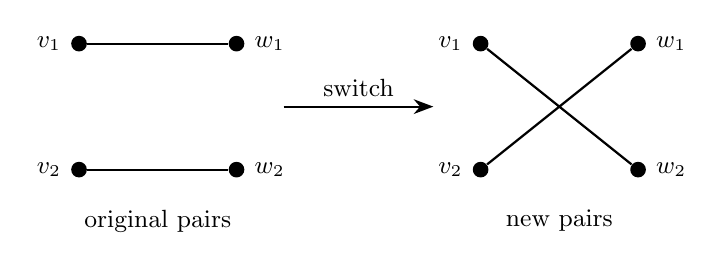
\begin{tikzpicture}[x=1cm,y=1cm,
 vertex/.style={circle,fill=black,inner sep=2pt},
 edge/.style={line width=.8pt},every node/.style={font=\small}]
 \foreach \offset/\tag in {0/a,5.1/b}{
   \node[vertex,label=left:{$v_1$}] (\tag v1) at (\offset,1.6) {};
   \node[vertex,label=left:{$v_2$}] (\tag v2) at (\offset,0) {};
   \node[vertex,label=right:{$w_1$}] (\tag w1) at (\offset+2,1.6) {};
   \node[vertex,label=right:{$w_2$}] (\tag w2) at (\offset+2,0) {};
 }
 \draw[edge] (av1)--(aw1) (av2)--(aw2);
 \draw[edge] (bv1)--(bw2) (bv2)--(bw1);
 \draw[-{Stealth[length=2.5mm]},line width=.7pt] (2.6,.8)--(4.5,.8)
    node[midway,above] {switch};
 \node at (1,-.65) {original pairs};
 \node at (6.1,-.65) {new pairs};
\end{tikzpicture}

 \caption{A two-edge switch on an induced matching. The marked pairs
 \((v_1,w_1)\) and \((v_2,w_2)\) are replaced by
 \((v_1,w_2)\) and \((v_2,w_1)\). Each endpoint loses one edge and gains
 one edge, so its degree is preserved. All other graph edges remain in
 place, and the marked list records the new pairs. The same exchange
 reverses the operation.}
 \label{fig:two-edge-switch}
\end{figure}
With probability \(1-O_k(n^{-1})\), the \(2k\) sampled endpoints are
distinct and the only graph edges among them are the sampled pairs.
This follows directly from fixed degree and conditional independence
of the edge samples. Restrict temporarily to this event. Exchange the
ending vertices of the first two pairs and update their entries in the
edge list. The operation is a bijection of the restricted graph/list
space, and all its elements have the same probability. In particular
the switched data, denoted by hats, satisfy
\eqref{eq:lim-concentration-implication} with the same failure bound.
The restriction itself is preserved by the switch.

The adjacency update has bounded rank. The eigenvalue counting
functions before and after the update consequently differ by a bounded
amount. Integrating their difference against the derivative of
\((t-z)^{-1}\) gives
\begin{equation}\label{eq:lim-rank-trace}
 |\widehat m_n(z)-m_n(z)|\le \frac C{\Im z}.
\end{equation}
This calculation is in the microscopic spectral variable; equivalently,
\(m_n(z)=\Tr(n(A-E)-z)^{-1}\).

Write the first two oriented pairs as \((v_1,w_1),(v_2,w_2)\), and put
\[
 f_1=\frac{e_{v_1}-e_{v_2}}{\sqrt2},\qquad
 f_2=\frac{e_{w_1}-e_{w_2}}{\sqrt2},\qquad F=(f_1,f_2).
\]
The switch adds \(F B F^{\mathsf T}\), where
\[
 B=\begin{pmatrix}0&-2\\-2&0\end{pmatrix}.
\]
Let \(U=F^{\mathsf T}(A-E-z/n)^{-1}F\), and define \(\widehat U\) using
the switched graph but the same old columns \(F\). The resolvent
identity yields
\begin{equation}\label{eq:lim-switch-identity}
 (I+UB)\widehat U=U.
\end{equation}
Suppose now that \(m=m_n(z)\) lies in a fixed bounded range.
Equations~\eqref{eq:lim-concentration-implication} and
\eqref{eq:lim-rank-trace}, applied to both data sets with a sufficiently
large trace threshold, give
\begin{equation}\label{eq:lim-switch-compressions}
 U=\begin{pmatrix}m&q\\q&m\end{pmatrix}
       +O((\Im z)^{-c_2}),\qquad
 \widehat U=\begin{pmatrix}m&-q\\-q&m\end{pmatrix}
       +O((\Im z)^{-c_2}),\qquad
 q=\frac{1+E m}{d}.
\end{equation}
The sign in the second matrix comes from expressing the updated edge
list in the old columns: the right difference column is negated.
The off-diagonal entries of \eqref{eq:lim-switch-identity} now imply
\begin{equation}\label{eq:lim-scalar-equation}
 q^2-q-m^2=O((\Im z)^{-c_2}).
\end{equation}
As a quadratic in \(m\), its exact left side has simple conjugate roots
in the strict bulk. By Lemma~\ref{lem:tree-identities}, the upper root is
\(m_*\). The lower root stays a fixed distance from every \(m\) with
\(\Im m\ge0\). Hence, throughout the bounded range,
\begin{equation}\label{eq:lim-scalar-stability}
 m_n(z)=m_*+O((\Im z)^{-c_2}).
\end{equation}

\paragraph{Closing the descent.}
There is no a priori trace assumption at a lower step. Instead, if
\(\eta/2\le\eta'\le\eta\), the resolvent sum gives
\begin{equation}\label{eq:lim-halving-bound}
 \begin{split}
 |m_n(s+\mathrm i\eta')-m_n(s+\mathrm i\eta)|
 &\le \frac{\eta-\eta'}{\eta'}\Im m_n(s+\mathrm i\eta)\\
 &\le \Im m_n(s+\mathrm i\eta).
 \end{split}
\end{equation}
Indeed
\(|x-s-\mathrm i\eta'|\ge(\eta'/\eta)|x-s-\mathrm i\eta|\)
term by term. Choose a fixed trace range containing the initial value
and every possible next-step value in \eqref{eq:lim-halving-bound}
when the preceding value is within \(1\) of \(m_*\). Enlarge it once
more for the switched trace using \eqref{eq:lim-rank-trace}. Finally
take the terminal height \(y\) sufficiently large that
\eqref{eq:lim-scalar-stability} returns a value within \(1\) of \(m_*\).
Induction down the heights proves the required trace bounds and the
endpoint estimates at every step.

Combining the two concentration failure bounds, and decreasing the
final exponent from \(c_2\) to a smaller \(\xi>0\), absorbs the fixed
constants into the threshold \(y^{-\xi}\). This proves
\eqref{eq:lim-endpoint-control}. All constants are independent of \(s\):
the only additional restriction was that \(S\) eventually exceed a
fixed multiple of \(|s|+y+1\), which holds before the limit for every
fixed \(s,y\).
\end{proof}

\subsection{The limiting marked process}

We now take subsequential limits in \(n\). The probability estimates
above will be used again only after this limit has been taken. For a
locally finite point measure \(\nu=\sum_j\delta_{x_j}\), a principal
value below always means the symmetric position truncation
\(\lim_{R\to\infty}\sum_{|x_j|\le R}\).

\begin{proposition}[Microscopic limits]\label{prop:microscopic-limit}
From every sequence of admissible sizes tending to infinity one can
extract a subsequence along which
\[
 \bigl(\nu_n,m_n,(M_{n,k})_{k\ge1}\bigr)
 \ \Longrightarrow\
 \bigl(\nu,m,(M_k)_{k\ge1}\bigr)
\]
jointly, in the local vague topology for the point measures and the
compact-open topology on the upper half-plane for the analytic
functions. The limiting point measure \(\nu=\sum_j\delta_{x_j}\) is
locally finite, with multiplicities permitted. There are deterministic
\(\xi,\chi>0\), depending only on \(d,E\), such that the following
properties hold.

For every fixed \(0<\delta<1\), almost surely for all sufficiently
large \(R\),
\begin{equation}\label{eq:mesoscopic-limit}
 m(e+\mathrm i u)=m_*+O(u^{-\xi}),
 \qquad |e|\le R,\quad R^\delta\le u\le R^2,
\end{equation}
and, almost surely,
\begin{equation}\label{eq:discrepancy}
 \nu([v,w])=\rho(w-v)+O(R^{1-\chi}),
 \qquad -R\le v\le w\le R,\quad R\longrightarrow\infty.
\end{equation}
The constants and starting values of \(R\) in these almost sure
statements may depend on the sample and on \(\delta\), but the exponents
are deterministic.

On a possible extension of the probability space, for every fixed
\(k\) there are standard Gaussian vectors \(g_j\in\R^{2k}\), independent
over \(j\) conditionally on \(\nu\), such that
\begin{equation}\label{eq:marked-representation}
 \begin{split}
  m(z)&=m_{\rm r}+\PV\sum_j\frac1{x_j-z},\\
  M_k(z)&=K_k(m_{\rm r})
       +\PV\sum_j
       \frac{C_k^{1/2}g_jg_j^{\mathsf T}C_k^{1/2}}{x_j-z}.
 \end{split}
\end{equation}
These representations are consistent as \(k\) increases by retaining
the first \(k\) edge channels. A separate Gaussian mark is assigned to
each occurrence of a repeated point. The principal values converge
locally uniformly on the upper half-plane, and
\(\Im M_k(z)\) is positive definite there, almost surely simultaneously
for every finite \(k\) and every \(z\) with \(\Im z>0\).
\end{proposition}

\begin{proof}
\leavevmode
\paragraph{Tightness.}
For fixed \(L,y>0\), positivity gives
\[
 \nu_n([-L,L])\le \frac{L^2+y^2}{y}\Im m_n(\mathrm i y).
\]
Proposition~\ref{prop:endpoint-control}, with \(y\) a sufficiently
large fixed number, therefore proves tightness of the local counts.
It also proves compact-open tightness of the analytic functions.
The choice of \(y\) is made separately for each probability tolerance:
choose it so that the bound \(C_{k,D}y^{-D}\) is below that tolerance,
and then take \(n\) large. A single height is not required to handle
all tolerances. Finitely many initial sizes do not affect tightness.
Here is a direct way to see the needed compact bounds. For a scalar
resolvent sum \(f\) with nonnegative residues, and a compact set
\(\mathcal K\) in the upper half-plane,
\[
 \Im f(z)\le C_{\mathcal K,y}\Im f(\mathrm i y),
 \qquad
 |f(z)-f(\mathrm i y)|
 \le C_{\mathcal K,y}\Im f(\mathrm i y),
 \qquad z\in\mathcal K.
\]
Both inequalities follow by comparing the corresponding kernels on
the real line. Apply them to \(m_n\), and to the real quadratic forms
of \(M_{n,k}\); polarization controls the matrix entries. Thus bounded
values at \(\mathrm i y\) give uniform bounds on each fixed compact,
and Cauchy's estimates give equicontinuity on smaller compacts.

We may consequently extract the asserted joint limit by tightness,
first on growing compact sets and finitely many channel dimensions,
and then diagonally. Local vague limits with locally bounded counts
are point measures with integer multiplicities. Limits of the
analytic functions have nonnegative imaginary parts in the same
scalar or matrix sense.

\paragraph{Conditional Gaussian marks on compact intervals.}
Choose nested compact position intervals exhausting \(\R\), with
boundaries almost surely uncharged by \(\nu\). Such deterministic
boundaries can be chosen because the set of points with positive
probability of carrying an atom is countable. On each interval,
truncate its point count at a fixed integer. Order the prelimit
indices using graph data alone, resolving ties by the chosen
eigenbasis ordering. The positions and the corresponding marks are
tight: their number is bounded, and the conditional second-moment
estimates of Proposition~\ref{prop:edge-moments} control the marks.
Extract these marked lists together with the preceding limit.

For completeness, fixed-order moment matching suffices here even
though the selected indices depend on the graph. For any fixed
number of indices, the approximation is uniform over their choices.
By a diagonal selection of the graph exceptional events, one may
require that an increasing finite collection of moment orders match
with errors tending to zero, on events of probability tending to one.
More explicitly, for each fixed list length and \(k\), choose integers
\(J_n\to\infty\) sufficiently slowly that all orders at most \(J_n\)
have errors at most \(J_n^{-1}\) on a common graph event of probability
at least \(1-J_n^{-1}\). This uses only finitely many fixed-order
assertions at each stage, not a uniform growing-order estimate.
If the conditional mark laws failed to approach their product
Gaussian law in a metric for weak convergence, one could select a
deterministic sequence of graphs and index lists with this failure
while every fixed moment converged. Tightness and moment
determinacy of the Gaussian law contradict that selection.
Thus conditional weak convergence is uniform over these bounded
lists.

Bounded Lipschitz tests, first with the list length truncated, now
show that the same joint limit is obtained by assigning independent
Gaussian marks to the prelimit positions independently of the graph.
Letting the truncation increase identifies the conditional marking
law given the full unmarked process \(\nu\). The covariance in
\(2k\) endpoint coordinates is \(C_k\). At a repeated limiting
position the list can be retained on an extension of the probability
space, with a separate independent mark for each multiplicity;
its summed outer product does not require an intrinsic ordering of
the tied points. Diagonal extraction in the intervals and in \(k\)
gives consistent marks
\begin{equation}\label{eq:lim-gaussian-marks}
 b_j=C_k^{1/2}g_j
\end{equation}
for all finite channel dimensions.

\paragraph{Removing imaginary tails.}
The convergence of compact marked sums alone does not yet identify
the full resolvents. For fixed \(z\) in the upper half-plane and
large \(L\), the scalar kernels satisfy, when \(|x|>L\),
\begin{equation}\label{eq:lim-tail-domination}
 \Im\frac1{x-z}
 +\left|\frac1{x-z}-\frac1{x-\mathrm i}\right|
 \le \frac{C_z}{L}\Im\frac1{x-\mathrm i L}.
\end{equation}
The constants can be uniform for \(z\) in a fixed compact set.
For matrix sums use positivity of the residues and bound the norm
by the trace of the corresponding positive imaginary part.
Proposition~\ref{prop:endpoint-control} shows that these traces at
\(\mathrm i L\) are tight as \(L\) tends to infinity, after taking
the upper limit in \(n\). The prefactor \(L^{-1}\) in
\eqref{eq:lim-tail-domination} therefore removes the tails in
probability. Compact marked sums already converge, so
\begin{equation}\label{eq:lim-difference-identities}
 \begin{split}
  \Im m(z)&=\sum_j\Im\frac1{x_j-z},\\
  m(z)-m(\mathrm i)
    &=\sum_j\left(\frac1{x_j-z}-\frac1{x_j-\mathrm i}\right),\\
  \Im M_k(z)&=\sum_j b_jb_j^{\mathsf T}
                            \Im\frac1{x_j-z},\\
  M_k(z)-M_k(\mathrm i)
    &=\sum_j b_jb_j^{\mathsf T}
               \left(\frac1{x_j-z}-\frac1{x_j-\mathrm i}\right).
 \end{split}
\end{equation}
One may establish these identities first at countably many
arguments and then use positivity and continuity. The imaginary
sums and the sums of absolute values of the difference kernels are
finite. In particular no imaginary spectral mass, including a
linear Herglotz term, is lost at infinity. Real additive constants
are not excluded by this argument and will be identified below.

\paragraph{Uniform bounds after the microscopic limit.}
At every fixed \(s+\mathrm i y\),
Proposition~\ref{prop:endpoint-control} passes to the limit by the
portmanteau inequality for the open event where its error exceeds
the stated threshold. Its constants remain independent of the
fixed real part \(s\). Decrease \(\xi\) if necessary so that
\(\xi<1\).

Fix \(0<\delta<1\). In a padded region
\[
 |e|\le 2R,\qquad \tfrac12 R^\delta\le u\le 2R^2
\]
take a unit grid. There are \(O(R^3)\) grid points. For each fixed
dyadic \(R\), this is a finite collection of arguments in the exact
limiting law. The failure probability from
\eqref{eq:lim-endpoint-control} is at most
\(C R^{3-\delta D}\). Choose \(D\) sufficiently large and apply
Borel--Cantelli over dyadic \(R\).
The kernel identities in \eqref{eq:lim-difference-identities} give
\[
 |m'(z)|\le \frac{\Im m(z)}{\Im z}.
\]
Imaginary parts at arguments within bounded distance and comparable
height are comparable by their positive kernels. The error in
filling the unit grid is consequently \(O(1/u)\). Padding allows
all sufficiently large \(R\), not just dyadic values. This proves
\eqref{eq:mesoscopic-limit}. The limit in \(n\) preceded the growing
grid argument; no finite-\(n\) uniform estimate on expanding real
windows has been used. A countable set of \(\delta\)'s implies all
the stated fixed-\(\delta\) conclusions, by slightly decreasing
\(\delta\) when necessary.

\paragraph{From the Poisson transform to counts.}
Equation~\eqref{eq:mesoscopic-limit} first gives
\(\nu([-R,R])=O(R)\), by evaluating \(\Im m(\mathrm i R)\).
For \(-R\le v\le w\le R\), integrate
\(\pi^{-1}\Im m(e+\mathrm i\sqrt R)\) over \(e\in[v,w]\).
The result is
\[
 \rho(w-v)+O(R^{1-\xi/2}).
\]
To compare it with the sharp count, put
\[
 P_{v,w}(x)=\frac1\pi
   \int_v^w\frac{\sqrt R}{(x-e)^2+R}\dd e.
\]
The number of points within distance \(R^{3/4}\) of either
endpoint is \(O(R^{3/4})\): use
\eqref{eq:mesoscopic-limit} at that endpoint and height
\(R^{3/4}\). For points of \([-2R,2R]\) outside these two strips,
\[
 |P_{v,w}(x)-\boldsymbol 1_{[v,w]}(x)|=O(R^{-1/4}).
\]
Their total error is \(O(R^{3/4})\), since the number of points is
\(O(R)\). Finally, for \(|x|>2R\),
\(P_{v,w}(x)\le C R^{3/2}/x^2\); the linear count bound and dyadic
summation make this contribution \(O(\sqrt R)\).
These estimates are uniform in \(v,w\), and prove
\eqref{eq:discrepancy} for any sufficiently small deterministic
\[
 0<\chi<\min(1/4,\xi/2).
\]
The estimates also show that endpoint conventions have no effect
on the stated error bound.

At this point the limiting positions have a deterministic density
with a power-saving count error, and all finite spectral residues
have been identified. It remains to determine the real constants
that the compact convergence did not see.

\paragraph{Scalar principal values and their constant.}
Partial summation in \eqref{eq:discrepancy} gives, almost surely,
\begin{equation}\label{eq:lim-position-tails}
 \PV\sum_{|x_j|>R}\frac1{x_j}=O(R^{-\chi}),
 \qquad
 \sum_{|x_j|>R}\frac1{x_j^2}=O(R^{-1}).
\end{equation}
Only large \(R\) is involved, so possible points at zero do not
enter these expressions. To see the first assertion, apply the
count discrepancy separately on the positive and negative
half-lines; their leading density terms cancel in the symmetric
sum, and integration of \(O(t^{1-\chi})/t^2\) leaves
\(O(R^{-\chi})\). The second assertion follows directly from the
linear count bound.

Thus
\[
 S_\nu(z)=\PV\sum_j\frac1{x_j-z}
\]
exists locally uniformly and is analytic. Comparison with the
constant-density measure gives
\begin{equation}\label{eq:lim-pv-large-height}
 S_\nu(\mathrm i R)=\mathrm i\pi\rho+o(1).
\end{equation}
Indeed, on each half-line the counting error is
\(O(1+|v|^{1-\chi})\). Partial summation bounds its contribution
by a constant times
\[
 \int_0^\infty\frac{1+v^{1-\chi}}{v^2+R^2}\dd v=o(1),
\]
whereas the symmetric transform of constant density is
\(\mathrm i\pi\rho\).
By \eqref{eq:lim-difference-identities}, \(m-S_\nu\) is a constant
function, and its imaginary part is zero. Equations
\eqref{eq:mesoscopic-limit} and \eqref{eq:lim-pv-large-height}
identify that real constant as \(m_{\rm r}\).

\paragraph{Marked principal values and their constant.}
Fix \(k\) and condition on \(\nu\). Set
\[
 Z_j=b_jb_j^{\mathsf T}-C_k.
\]
These matrices are independent and centered, with bounded
second moments depending only on \(k,d,E\). The series
\(\sum_j Z_j/(x_j-\mathrm i)\), ordered by increasing \(|x_j|\),
converges almost surely entrywise by square summability and
independence. Also, conditionally almost surely,
\[
 \sum_{|x_j|>1}\frac{\|Z_j\|}{x_j^2}<\infty,
\]
because its conditional expectation is finite by
\eqref{eq:lim-position-tails}. Consequently the corresponding
difference series between \(z\) and \(\mathrm i\) converges
absolutely and locally uniformly. Together with the scalar
principal value this proves local uniform convergence of
\[
 S_{k,\nu}(z)=\PV\sum_j\frac{b_jb_j^{\mathsf T}}{x_j-z}.
\]

The linear count bound also gives
\[
 \sum_j|x_j-\mathrm i R|^{-2}=O(R^{-1}).
\]
Thus every entry of the centered marked series at
\(\mathrm i R\) has conditional second moment \(O(R^{-1})\),
with a sample-dependent constant. It follows that
\[
 S_{k,\nu}(\mathrm i R)
 \longrightarrow \mathrm i\pi\rho\,C_k
 \quad\hbox{in probability}.
\]
The limiting version of Proposition~\ref{prop:endpoint-control}
gives \(M_k(\mathrm i R)\to K_k(m_*)\) in probability. On the
other hand \eqref{eq:lim-difference-identities} shows that
\(M_k-S_{k,\nu}\) is almost surely constant in \(z\).
That constant must therefore equal
\[
 K_k(m_*)-\mathrm i\pi\rho\,C_k=K_k(m_{\rm r})
\]
almost surely. This proves both identities in
\eqref{eq:marked-representation}.

Finally, \eqref{eq:discrepancy} supplies infinitely many points,
and \(C_k\) is positive definite. Any \(2k\) independently
Gaussian marks span \(\R^{2k}\) almost surely. Their positive
contributions to the imaginary-part sum in
\eqref{eq:lim-difference-identities} make \(\Im M_k(z)\) positive
definite for every \(z\) in the upper half-plane on the same
event. Countability of the channel dimensions completes the
simultaneous assertion.
\end{proof}

\section{Continuous switches and Gaussian insertion}\label{sec:switching}

We work with a microscopic subsequential law supplied by
Proposition~\ref{prop:microscopic-limit}. Its endpoint marks are Gaussian,
whereas genuine graph switches preserve its law. Reversible switches
underlie the random-regular-graph comparison framework of
\citet[Section~3]{BauerschmidtEtAl}. We combine this finite-graph symmetry
with the Gaussian marks to obtain exact orthogonal switching symmetries.
We then use many small orthogonal switches to represent the same
point-process law as a limit of finite matrices with added GOE noise.

\subsection{From permutations to orthogonal switches}

Fix \(k\ge2\), and write \(M=M_k\). For \(O\in O(k)\), define the real matrices
\begin{equation}\label{eq:sw-definitions}
 D_O=\begin{pmatrix}\Id_k&0\\0&O\end{pmatrix},
 \qquad
 B_O=D_OJ_kD_O^\top-J_k.
\end{equation}
In particular, \(B_O\) is symmetric. For an analytic symmetric matrix function
\(M\) with positive definite imaginary part, put
\begin{equation}\label{eq:sw-transformation}
 \mathcal T_O(m,M)=
 \left(
 m-\partial_z\log\det(\Id_{2k}+B_OM),\
 D_O^\top(M^{-1}+B_O)^{-1}D_O
 \right).
\end{equation}
Only the logarithmic derivative is used, so no choice of logarithm is needed.
These expressions are well defined: \(M\) is invertible and
\[
 \Im(M^{-1})=-M^{-*}(\Im M)M^{-1}<0.
\]
Thus \(M^{-1}+B_O\) is invertible, and its inverse again has positive definite
imaginary part.

\begin{proposition}[Continuous switching symmetry]
\label{prop:continuous-switching}
For every fixed \(k\ge2\) and every \(O\in O(k)\), the joint analytic-function
law of \((m,M_k)\) is invariant under \(\mathcal T_O\).
\end{proposition}

\begin{proof}
First suppose that \(O\) is a permutation matrix. In a finite graph, let
\(W=W_{n,k}\) contain the starting endpoint columns followed by the ending
endpoint columns of the \(k\) sampled oriented edges. Except with probability
\(O_k(n^{-1})\), all endpoints are distinct and their induced subgraph is
exactly the marked matching. On this event,
\[
 A\longmapsto A+WB_OW^\top,\qquad W\longmapsto WD_O
\]
permutes the pairing between the two endpoint lists. The resulting graph is
simple and \(d\)-regular. Its marked list has the same restriction, and the
inverse permutation recovers the input. Every graph with its ordered list
has the same joint weight, so this bijection preserves the restricted law.

Write \(R(z)=(A-E-z/n)^{-1}\). The determinant and inverse identities for
finite-rank perturbations give
\begin{align*}
 \widehat m_n(z)
 &=m_n(z)-\partial_z\log\det(\Id_{2k}+B_OM_{n,k}(z)),\\
 \widehat M_{n,k}(z)
 &=D_O^\top(M_{n,k}(z)^{-1}+B_O)^{-1}D_O.
\end{align*}
Indeed \(m_n=n^{-1}\Tr R\), and differentiation in \(z\) supplies exactly
this factor \(n^{-1}\). The formulas also follow without requiring
invertibility of the prelimit compression by using
\((\Id+M_{n,k}B_O)^{-1}M_{n,k}\). In the limit, the positive definite
imaginary part already established makes the inverse formula regular.
Compact-open convergence of analytic functions also gives convergence of
their derivatives. We may therefore pass to the limit, proving the
proposition for permutation matrices.

Next let \(U\in O(k)\), and set \(Q_U=\diag(U,U)\).
The matrices \(C_k\) and \(K_k(m_{\rm r})\) commute with \(Q_U\).
The Gaussian representation~\eqref{eq:marked-representation} consequently
shows that
\[
 \mathcal R_U(m,M)=(m,Q_U^\top M Q_U)
\]
preserves the joint law. This assertion follows even conditionally on
\(\nu\), but we will need switching invariance only unconditionally.
Since \(Q_UD_OQ_U^\top=D_{UOU^\top}\) and
\(Q_UB_OQ_U^\top=B_{UOU^\top}\), the inverse and determinant formulas give
\[
 \mathcal R_U^{-1}\circ\mathcal T_O\circ\mathcal R_U
       =\mathcal T_{UOU^\top}.
\]
Thus the law is invariant under every orthogonal conjugate of a
permutation switch.

Finally, the switching maps form an action:
applying \(\mathcal T_O\) and then \(\mathcal T_{O'}\) gives
\(\mathcal T_{OO'}\). To check this directly, observe that
\begin{equation}\label{eq:sw-composition}
 B_{OO'}=B_O+D_OB_{O'}D_O^\top,\qquad D_{OO'}=D_OD_{O'}.
\end{equation}
Successive inverse updates therefore give the asserted second component.
The determinant ratios for the two updates multiply, which gives the first
component after logarithmic differentiation. A transposition is a
hyperplane reflection. Its orthogonal conjugates are all hyperplane
reflections, and their finite products generate \(O(k)\). The proposition
follows.
\end{proof}

\subsection{The finite Gaussian model}

Fix a discrepancy exponent \(0<\chi<1/4\) from
\eqref{eq:discrepancy}. We use \(r\) planar rotations, each through a
small angle \(\theta\), with aggregate variance of order
\(T=r\theta^2\). The position cutoff \(K\) specifies the finite block
that will receive GOE noise. A much larger temporary cutoff \(L\)
first turns the principal-value resolvent into a finite matrix.
We let \(T\) grow slowly relative to \(K\), and \(K\) slowly relative
to \(r\), so that deleting the outer positions and replacing the
individual summands both have vanishing errors. Choose once and for all
\begin{equation}\label{eq:sw-parameters}
 0<\tau<\frac{\chi}{100000},\qquad
 k=2r,\quad K=r^{1/100},\quad T=r^\tau,\quad
 \theta=\sqrt{T/r},\quad L=r^{100/\chi},
 \qquad r\in\N.
\end{equation}
For each \(r\), take \(O=O_r\) to be the direct sum of \(r\) planar rotations
of angle \(\theta\). Write \(B=B_{O_r}\) and \(M^0=K_k(m_{\rm r})\).
The coefficient below absorbs the constant \(M^0\) in the marked
resolvent when the first-cut argument converts the update into an
additive perturbation.
For all sufficiently large \(r\), the real symmetric matrix
\begin{equation}\label{eq:sw-coefficient}
 \Gamma_r=C_k^{1/2}(B^{-1}+M^0)^{-1}C_k^{1/2}
\end{equation}
is well defined. In fact the singular values of \(B\) are all
\(2|\sin(\theta/2)|\), and \(\|M^0\|\) is bounded independently of \(r\).
Let \(\beta\) be a diagonal matrix of eigenvalues of \(\Gamma_r\), and define
\begin{equation}\label{eq:sw-moments}
 s_1=\Tr\beta,\qquad s_2=\Tr\beta^2.
\end{equation}
These quantities are deterministic.

Index the limiting positions with multiplicity, and put
\[
 I=\{j:|x_j|\le K\},\qquad q_*=|I|,\qquad
 D_I=\diag(x_j:j\in I).
\]
Conditional on \(\nu\), let \(\mathcal W\) be a raw GOE matrix of size \(q_*\):
its off-diagonal entries have variance \(1\), and its diagonal entries have
variance \(2\). It is independent of \(\nu\), apart from its dimension. Define
\begin{equation}\label{eq:sw-inserted-matrix}
 H_r=D_I+s_1\Id_{q_*}+\sqrt{s_2}\,\mathcal W.
\end{equation}
An empty \(I\) gives an empty matrix and zero trace; almost surely this case
does not occur for large \(r\), by \eqref{eq:discrepancy}.

\begin{proposition}[Gaussian insertion]\label{prop:gaussian-insertion}
The coefficients in \eqref{eq:sw-moments} satisfy
\begin{equation}\label{eq:sw-coefficient-bounds}
 \|\beta\|\le C\theta,\qquad
 cT\le s_2\le CT,\qquad |s_1|\le CT,
\end{equation}
with deterministic positive constants. Moreover, as \(r\to\infty\),
\begin{equation}\label{eq:sw-trace-limit}
 m_{\rm r}+\Tr(H_r-z)^{-1}
 \ \Longrightarrow\ m(z)
\end{equation}
jointly at every finite list of points \(z\in\C_+\), and the unscaled
eigenvalue point measure of \(H_r\) converges locally vaguely in law to
\(\nu\). Both convergences are unconditional.

More precisely, generate the Gaussian marks of \(M_k\) conditionally on
\(\nu\), separately for each \(r\), and write
\[
 \mathcal S_r(z)
 =m(z)-\partial_z\log\det(\Id_{2k}+BM_k(z)).
 \]
For almost every \(\nu\), expectations of every bounded smooth function with
bounded derivatives of finitely many real and imaginary trace values differ
by \(o(1)\) when
\(m_{\rm r}+\Tr(H_r-z)^{-1}\) is replaced by \(\mathcal S_r(z)\).
This is a conditional approximation assertion, not conditional switching
invariance.
\end{proposition}

We prove the approximation in three steps. Cutting the principal-value
sums at \(L\) converts the switched trace into the trace of a finite
diagonal matrix perturbed by \(4r\) rank-one terms built from Gaussian
vectors. We then
delete the positions between \(K\) and \(L\), using the signed
principal-value tail cancellation to control the Schur complement.
Finally, on the retained block of order \(K\), a summand-by-summand
replacement turns the perturbation into a scalar shift plus GOE noise
with the same mean and entry covariances.

The graph size \(n\) has already tended to infinity, and
Proposition~\ref{prop:continuous-switching} is exact for every fixed \(k\).
We now let \(r\), and hence \(k=2r\), grow within that limiting law.
No growing-dimensional version of the prelimit eigenvector moment estimates
is needed. For the approximation estimates below, condition on any \(\nu\)
in the probability-one event on which
\eqref{eq:mesoscopic-limit}--\eqref{eq:marked-representation} hold.
Constants may depend on this conditioning input and on a fixed finite list
of spectral parameters. Probability notation in the intermediate estimates
refers to the Gaussian marks.

\subsection{A first cut at a large distance}

We first convert a switched trace into the trace of a finite random matrix.
The elementary consequences of \eqref{eq:discrepancy} that we use are
\begin{equation}\label{eq:sw-tail-sums}
 \nu([-R,R])=2\rho R+O(R^{1-\chi}),\qquad
 \left|\PV\sum_{|x_j|>R}\frac1{x_j}\right|=O(R^{-\chi}),
 \qquad
 \sum_{|x_j|>R}\frac1{x_j^2}=O(R^{-1}).
\end{equation}
The last two follow by partial summation on the positive and negative
half-lines, retaining their constant-density terms together in the
principal-value sum.

Cut the representation of \(M=M_k\) at \(L\), keeping the constant \(M^0\):
\[
 M_L(z)=M^0+
 \sum_{|x_j|\le L}
 \frac{C_k^{1/2}g_jg_j^\top C_k^{1/2}}{x_j-z}.
\]
For fixed \(z\in\C_+\),
\begin{equation}\label{eq:sw-first-tail}
 \|M-M_L\|+\|M'-M_L'\|=O_{\PP}(r^2L^{-\chi}),
 \qquad \|M'\|=O_{\PP}(r^2).
\end{equation}
Here is the dimension dependence in these bounds. The deterministic mean
tail is \(O(L^{-\chi})C_k\) for \(M\), and \(O(L^{-1})C_k\) for its
derivative. Each entry of the centered Gaussian tail has variance
\(O(L^{-1})\), using \eqref{eq:sw-tail-sums}; the derivative has a smaller
variance. There are \((4r)^2\) entries, so the Hilbert--Schmidt estimate gives
\(O_{\PP}(rL^{-1/2})\). This is smaller than the bound displayed in
\eqref{eq:sw-first-tail}. For \(M'\), the absolute scalar weights sum to a
finite constant depending on \(z,\nu\), and the expected sum of the norms of
the positive rank-one matrices is \(O(r)\). The stated \(O_{\PP}(r^2)\) bound is
therefore sufficient and conservative.

We also need a lower bound on the imaginary parts in order to use inverse
updates stably. Keep only the indices \(|x_j|\le r^4\). Their number is
asymptotic to \(2\rho r^4\), and their scalar weights in \(\Im M(z)\) are at
least \(c_z r^{-8}\). If \(b_j=C_k^{1/2}g_j\), Gaussian fourth moments give
\[
 \EE\left\|
 \frac1{|\{j:|x_j|\le r^4\}|}
 \sum_{|x_j|\le r^4}b_jb_j^\top-C_k
 \right\|_{\HS}^2=O(r^{-2}).
\]
Since the smallest eigenvalue of \(C_k\) is bounded below independently of
\(k\), both \(M\) and \(M_L\) consequently satisfy
\begin{equation}\label{eq:sw-imaginary-lower}
 \Im M(z)\ge r^{-5}\Id_{4r},\qquad
 \Im M_L(z)\ge r^{-5}\Id_{4r}
\end{equation}
with probability tending to one. We used \(L\gg r^4\) here.
As \(B^{-1}\) is real symmetric, \eqref{eq:sw-imaginary-lower} bounds the
norms of \((B^{-1}+M)^{-1}\) and \((B^{-1}+M_L)^{-1}\) by \(r^5\).

It follows that cutting both scalar and marked sums in
\[
 \mathcal S_r(z)=m(z)-\Tr(B^{-1}+M(z))^{-1}M'(z)
\]
costs \(o_{\PP}(1)\). To make the margin explicit, the marked tail in
\eqref{eq:sw-first-tail} is \(O_{\PP}(r^{-98})\). The inverse identity bounds
the two trace errors by
\[
 O_{\PP}\bigl(r\cdot r^5\cdot r^{-98}\bigr)
 +O_{\PP}\bigl(r\cdot r^{10}\cdot r^{-98}\cdot r^2\bigr)
 =O_{\PP}(r^{-92}+r^{-85}).
\]
The scalar tail is \(O(L^{-\chi})\).

Let \(D=\diag(x_j:|x_j|\le L)\).
Diagonalizing the real symmetric coefficient \(\Gamma_r\), and rotating
the independent Gaussian row vectors in channel space, gives a matrix
\(\mathcal G\) of independent standard real Gaussian entries with \(4r\)
columns. The finite-rank inverse identity now yields
\begin{equation}\label{eq:sw-finite-matrix}
 \mathcal S_r(z)
 =m_{\rm r}+\Tr(D+A'-z)^{-1}+o_{\PP}(1),
 \qquad A'=\mathcal G\beta\mathcal G^\top .
\end{equation}
Indeed \(B^{-1}+M_L\) is the sum of \(B^{-1}+M^0\) and the marked
compression of \((D-z)^{-1}\), while its derivative is the compression of
\((D-z)^{-2}\). Woodbury's formula gives exactly the trace difference
in \eqref{eq:sw-finite-matrix}.

For completeness, the coefficient estimates
\eqref{eq:sw-coefficient-bounds} follow directly from this construction.
The identity
\[
 (B^{-1}+M^0)^{-1}=(\Id+BM^0)^{-1}B=B+O(\theta^2)
\]
holds in operator norm uniformly in \(r\). Every singular value of this
matrix is comparable to \(\theta\); conjugation by \(C_k^{1/2}\) preserves
this comparison. Since the dimension is \(4r\), we obtain
\(\|\beta\|=O(\theta)\) and \(s_2\asymp r\theta^2=T\). Finally,
\[
 s_1=\Tr(C_kB)+O(r\theta^2),\qquad
 \Tr(C_kB)=2p\,\Tr(O-\Id_k)=O(r\theta^2).
\]
This proves all three bounds, including the cancellation needed for
the mean \(s_1\).

\subsection{Removing the outer positions}

The finite matrix in \eqref{eq:sw-finite-matrix} still has order \(L\).
We next show that its outer positions can be deleted at the level of
resolvent traces. This is necessary before making a Gaussian replacement:
the available small-summand estimate will be applied only to the much
smaller block of order \(K\).

Let \(F=\{j:K<|x_j|\le L\}\), so that the indices of \(D\) split into \(I,F\).
Put
\begin{equation}\label{eq:sw-weights}
 h=T^2,\qquad U_I=(|D_I|+h)^{-1/2},\qquad
 U_F=|D_F|^{-1/2}.
\end{equation}
Partial summation using \eqref{eq:sw-tail-sums} gives
\begin{equation}\label{eq:sw-weight-bounds}
 \Tr U_I^2+\Tr U_F^2=O(\log r),\qquad
 \|U_I^2\|\le h^{-1},\quad \|U_F^2\|\le K^{-1}.
\end{equation}
For example, the inner sum is bounded by integrating the linear count
bound against \((|x|+h)^{-1}\); the far sum is treated in the same way
between \(K\) and \(L\). Both endpoints are fixed powers of \(r\).
In the following estimates, \(\operatorname{polylog}(r)\) denotes a fixed
power of \(\log r\), whose exponent may increase from one occurrence
to the next.

\begin{lemma}[Weighted block estimates]\label{sw:weighted-blocks}
For \(\mathcal A=I,F\), put \(a_I=h\), \(a_F=K\). With probability tending
to one,
\begin{equation}\label{eq:sw-bernstein}
 \left\|U_{\mathcal A}
       (A'_{\mathcal A\mathcal A}-s_1\Id)
       U_{\mathcal A}\right\|
 \le \operatorname{polylog}(r)
       \left(\sqrt{T/a_{\mathcal A}}+\theta\right).
\end{equation}
Moreover, for \(P_0=U_IA'_{IF}U_F\),
\begin{equation}\label{eq:sw-cross-block}
 \|P_0\|_{\HS}^2\le T\operatorname{polylog}(r)
\end{equation}
with probability tending to one.
\end{lemma}

\begin{proof}
The centered matrix in \eqref{eq:sw-bernstein} is a sum of independent
self-adjoint matrices
\[
 \sum_{\alpha=1}^{4r}\beta_{\alpha\alpha}
       (v_\alpha v_\alpha^\top-P),\qquad P=U_{\mathcal A}^2,
\]
where \(v_\alpha\) is Gaussian of covariance \(P\).
Its coefficients may have either sign. Gaussian fourth moments give
\begin{equation}\label{eq:sw-fourth-moment}
 \EE[(v_\alpha v_\alpha^\top)^2]
   =(\Tr P)P+2P^2.
\end{equation}
Truncate each original Gaussian column on the event that all its entries
have absolute value at most \(\log r\), and center the truncated summand.
There are only polynomially many entries, so this alters the matrices with
superpolynomially small probability. Gaussian tails also make the resulting
centering correction superpolynomially small.

Each truncated summand has norm at most
\[
 C\|\beta\|(\log r)^2\Tr P
 \le \theta\operatorname{polylog}(r).
\]
If \(X\) is a self-adjoint random matrix, then
\(\EE[(X-\EE X)^2]=\EE[X^2]-(\EE X)^2\le\EE[X^2]\).
Also truncating \(v_\alpha v_\alpha^\top\) by an event can only decrease
the expectation of its square in positive semidefinite order.
Thus \eqref{eq:sw-fourth-moment}, including for negative
\(\beta_{\alpha\alpha}\), bounds the matrix variance parameter by
\[
 C s_2(\Tr P)\|P\|
 \le \frac{T}{a_{\mathcal A}}\operatorname{polylog}(r).
\]
The bounded self-adjoint matrix Bernstein inequality
\citep[Theorem~1.4]{Tropp} gives, for a sum of independent centered
self-adjoint matrices of norm at most \(b\) and variance parameter
\(\sigma_{\rm mat}^2\), a two-sided tail bounded by
\[
 2|\mathcal A|\exp\left(
 -\frac{c t^2}{\sigma_{\rm mat}^2+bt}\right).
\]
Its dimension factor is polynomial in \(r\). Taking a sufficiently large
power of \(\log r\) in \(t\) proves \eqref{eq:sw-bernstein}.

For the cross block, independence of distinct Gaussian rows and direct
second-moment calculation give
\[
 \EE\|P_0\|_{\HS}^2
 =s_2(\Tr U_I^2)(\Tr U_F^2).
\]
Equation~\eqref{eq:sw-cross-block} follows from
\eqref{eq:sw-weight-bounds} and Markov's inequality, with one additional
logarithmic factor.
\end{proof}

Fix \(z\in\C_+\), and define
\[
 G_F=(D_F+A'_{FF}-z)^{-1},\qquad
 G_I=(D_I+A'_{II}-z)^{-1}.
\]
The next estimates control the influence of the far block even at the fixed
imaginary part \(\Im z\).

\begin{lemma}[Far block and Schur correction]\label{sw:schur}
Let
\[
 \delta_F=\operatorname{polylog}(r)
       \left(\frac{1+T}{K}+\sqrt{\frac TK}+\theta\right).
\]
Then
\begin{equation}\label{eq:sw-far-resolvent}
 \|U_F^{-1}(G_F-D_F^{-1})U_F^{-1}\|\le\delta_F=o(1)
\end{equation}
with probability tending to one, and \(\Tr G_F=o_{\PP}(1)\).
For \(\Sigma=A'_{IF}G_FA'_{FI}\),
\begin{equation}\label{eq:sw-schur-small}
 \|U_I\Sigma U_I\|=o_{\PP}(T^{-5}).
\end{equation}
\end{lemma}

\begin{proof}
Conjugating the matrix to be inverted by \(U_F\) gives
\[
 U_F(D_F+A'_{FF}-z)U_F
 =\operatorname{sign}(D_F)+U_F(A'_{FF}-z)U_F.
\]
The second term has norm at most \(\delta_F\), by
Lemma~\ref{sw:weighted-blocks}, the bound \(|s_1|=O(T)\), and
\eqref{eq:sw-weight-bounds}. Since \(\delta_F=o(1)\), a Neumann expansion
proves \eqref{eq:sw-far-resolvent}. In particular,
\(Q_F=U_F^{-1}G_FU_F^{-1}\) has bounded norm.
By \eqref{eq:sw-tail-sums},
\[
 \left|\sum_{j\in F}\frac1{x_j}\right|=O(K^{-\chi}),
 \qquad
 |\Tr(G_F-D_F^{-1})|
 \le\delta_F\Tr U_F^2=o(1).
\]
This proves the assertion about the far trace.

For the Schur correction, replacing \(G_F\) by \(D_F^{-1}\) costs at most
\begin{equation}\label{eq:sw-schur-replacement}
 \|P_0\|_{\HS}^2\delta_F
 \le T\operatorname{polylog}(r)\delta_F
\end{equation}
in the norm weighted on both sides by \(U_I\).
It remains to estimate
\(A'_{IF}D_F^{-1}A'_{FI}\).
Condition further on the inner Gaussian row block \(\mathcal G_I\), and set
\[
 Q=\mathcal G_I\beta^2\mathcal G_I^\top.
\]
The columns of \(A'_{IF}\), indexed by \(j\in F\), are then independent
centered Gaussian vectors \(a_j\) with covariance \(Q\).
Consequently
\begin{align*}
 \EE\left[\sum_{j\in F}\frac{a_ja_j^\top}{x_j}
       \,\middle|\,\mathcal G_I,\nu\right]
 &=Q\sum_{j\in F}\frac1{x_j},\\
 \Var\left(\sum_{j\in F}\frac{(a_j)_a(a_j)_b}{x_j}
       \,\middle|\,\mathcal G_I,\nu\right)
 &=(Q_{aa}Q_{bb}+Q_{ab}^2)
       \sum_{j\in F}\frac1{x_j^2}.
\end{align*}
Also
\(\EE[Q_{aa}^2\mid\nu]
 =s_2^2+2\Tr\beta^4=O(T^2)\).
Since \(Q\) is positive semidefinite,
\(|Q_{ab}|^2\le Q_{aa}Q_{bb}\); Cauchy--Schwarz bounds the remaining
second moments by \(O(T^2)\).
Multiplying entry \(a,b\) by \((U_I)_{aa}(U_I)_{bb}\), summing its second
moment over \(a,b\), and using \eqref{eq:sw-tail-sums} and
\eqref{eq:sw-weight-bounds}, we obtain
\[
 \EE\left\|
 U_IA'_{IF}D_F^{-1}A'_{FI}U_I
 \right\|_{\HS}^2
 \le C T^2(\log r)^2(K^{-2\chi}+K^{-1}).
\]
Markov's inequality therefore bounds this norm by
\(T\operatorname{polylog}(r)(K^{-\chi}+K^{-1/2})\) with probability
tending to one.

Combining this estimate with \eqref{eq:sw-schur-replacement} gives
\[
 \|U_I\Sigma U_I\|
 \le \operatorname{polylog}(r)\,O\left(
 TK^{-\chi}+TK^{-1/2}+\frac{T(1+T)}K
       +T\sqrt{T/K}+T\theta\right)
\]
with probability tending to one. After multiplication by \(T^5\), all
terms tend to zero by a fixed power of \(r\). For example, the three
potentially slow terms have exponents
\[
 6\tau-\frac{\chi}{100},\qquad
 \frac{13}{2}\tau-\frac1{200},\qquad
 \frac{13}{2}\tau-\frac12,
\]
respectively. They are negative under \eqref{eq:sw-parameters}; the terms
\(T^6K^{-1/2}\) and \(T^6(1+T)/K\) have still ample margins.
This proves \eqref{eq:sw-schur-small}.
\end{proof}

We now convert the small weighted Schur correction into a small trace
error. The fixed-height inner resolvent cannot be estimated directly from
\eqref{eq:sw-bernstein}; instead we first work at the larger height \(h=T^2\).

\begin{lemma}[Inner resolvent and trace cut]\label{sw:trace-cut}
For every fixed \(z\in\C_+\),
\begin{equation}\label{eq:sw-inner-resolvent}
 \|U_I^{-1}G_I(z)U_I^{-1}\|=O_{\PP}(h),
\end{equation}
and
\begin{equation}\label{eq:sw-second-cut}
 \Tr(D+A'-z)^{-1}
 =\Tr(D_I+A'_{II}-z)^{-1}+o_{\PP}(1).
\end{equation}
The same estimates hold jointly for a fixed finite list of \(z\)'s.
\end{lemma}

\begin{proof}
Every diagonal entry of \(U_I(D_I-ih)U_I\) has modulus at least
\(1/\sqrt2\). The added term has norm at most
\[
 \|U_IA'_{II}U_I\|
 \le C T/h+\operatorname{polylog}(r)
       \left(\sqrt{T/h}+\theta\right)=o(1)
\]
with probability tending to one. Hence
\[
 \|U_I^{-1}G_I(ih)U_I^{-1}\|\le C.
\]
The identity \(G_I(ih)^*G_I(ih)=h^{-1}\Im G_I(ih)\) now gives
\[
 \|G_I(ih)U_I^{-1}\|+\|U_I^{-1}G_I(ih)\|
 \le C h^{-1/2}.
\]
Alternatively the same mixed-weight estimates follow from the preceding
weighted inverse and \(\|U_I\|\le h^{-1/2}\).
Use the exact twice-iterated resolvent identity
\begin{align*}
 G_I(z)
 ={}&G_I(ih)+(z-ih)G_I(ih)^2\\
 &+(z-ih)^2G_I(ih)G_I(z)G_I(ih).
\end{align*}
The unweighted middle resolvent in the last term has norm at most
\((\Im z)^{-1}\). Conjugating the identity by \(U_I^{-1}\), the three
terms are bounded by
\[
 C,\qquad C|z-ih|/h,\qquad
 C|z-ih|^2/(h\Im z),
\]
respectively. This proves \eqref{eq:sw-inner-resolvent}.

The Schur complement formula for the full inverse has upper-left block
\(\widetilde G_I=(G_I^{-1}-\Sigma)^{-1}\).
Set \(R_I=U_I^{-1}G_IU_I^{-1}\) and \(S_I=U_I\Sigma U_I\).
Then
\[
 U_I^{-1}\widetilde G_IU_I^{-1}
 =(R_I^{-1}-S_I)^{-1}.
\]
By \eqref{eq:sw-inner-resolvent} and
\eqref{eq:sw-schur-small}, a Neumann expansion gives
\[
 \|U_I^{-1}\widetilde G_IU_I^{-1}\|=O_{\PP}(h),\qquad
 \|U_I^{-1}(\widetilde G_I-G_I)U_I^{-1}\|
 \le O_{\PP}(h^2)o_{\PP}(T^{-5})=o_{\PP}(T^{-1}).
\]
Multiplying the last bound by \(\Tr U_I^2=O(\log r)\) shows that their
traces differ by \(o_{\PP}(1)\).

The full block-inverse trace is
\[
 \Tr\widetilde G_I+\Tr G_F+
 \Tr\bigl(\widetilde G_IA'_{IF}G_F^2A'_{FI}\bigr).
\]
The far trace is \(o_{\PP}(1)\) by Lemma~\ref{sw:schur}.
For the last term recall \(Q_F=U_F^{-1}G_FU_F^{-1}\).
It has bounded norm, and
\[
 U_F^{-1}G_F^2U_F^{-1}=Q_FU_F^2Q_F,\qquad
 \|Q_FU_F^2Q_F\|=O_{\PP}(K^{-1}).
\]
No positivity is asserted for this complex square. The ordinary
operator-norm and Hilbert--Schmidt trace inequality instead gives
\begin{align*}
 \left|\Tr\bigl(\widetilde G_IA'_{IF}G_F^2A'_{FI}\bigr)\right|
 &\le
 \|U_I^{-1}\widetilde G_IU_I^{-1}\|\,
 \|P_0\|_{\HS}^2\,
 \|Q_FU_F^2Q_F\|\\
 &\le \operatorname{polylog}(r)\,O_{\PP}(T^3/K)=o_{\PP}(1).
\end{align*}
This proves \eqref{eq:sw-second-cut}. All estimates used the same Gaussian
matrices, so taking a finite union gives the joint assertion.
\end{proof}

\subsection{Gaussian replacement and convergence of point measures}

We have reduced the switched trace to an inner matrix of size
\[
 q_*=2\rho K+O(K^{1-\chi})\asymp K.
\]
Its perturbation is a sum of \(4r\) independent small rank-one matrices.
Only at this reduced size do we replace that sum by GOE noise.
We use the one-summand replacement and Taylor-expansion method of the
Lindeberg principle; see \citet{ChatterjeeLindeberg} for a general
formulation. The matrix estimate needed here is proved below.

\begin{lemma}[Gaussian replacement]\label{sw:lindeberg}
Conditional on almost every \(\nu\), bounded smooth tests with bounded
derivatives of finitely many trace values have expectation difference
\(o(1)\) between
\[
 D_I+A'_{II}
 \quad\hbox{and}\quad
 H_r=D_I+s_1\Id_{q_*}+\sqrt{s_2}\,\mathcal W.
\]
\end{lemma}

\begin{proof}
Write
\[
 A'_{II}-s_1\Id_{q_*}
 =\sum_{\alpha=1}^{4r}
 \beta_{\alpha\alpha}(g_\alpha g_\alpha^\top-\Id_{q_*}),
\]
where the \(g_\alpha\) are independent standard \(q_*\)-dimensional
Gaussian vectors. The covariance identity
\[
 \Cov(g_ag_b,g_cg_d)
 =\delta_{ac}\delta_{bd}+\delta_{ad}\delta_{bc}
\]
shows that \(gg^\top-\Id\) and a raw GOE matrix have the same entry
covariances. Their means are both zero. Thus replace the summands one at
a time by \(\beta_{\alpha\alpha}\mathcal W_\alpha\), with independent raw
GOE matrices \(\mathcal W_\alpha\). Negative coefficients are allowed:
both covariances are multiplied by \(\beta_{\alpha\alpha}^2\).

For either kind of summand \(X\),
\[
 \EE\|X\|^3\le C\theta^3q_*^3.
\]
For the rank-one term this follows from Gaussian moments of \(\|g\|^2\);
for the GOE term the Hilbert--Schmidt norm gives a sufficient bound.
Fix spectral parameters \(z_1,\ldots,z_b\in\C_+\), and a bounded smooth
test \(\Phi\) on the corresponding real and imaginary trace coordinates,
with bounded derivatives. For any real symmetric matrix \(A\), its
resolvents satisfy \(\|(A-z_\ell)^{-1}\|\le(\Im z_\ell)^{-1}\).
Differentiating the resolvent in a real symmetric direction \(\Delta\)
gives, for \(j=1,2,3\), a trace derivative bounded by
\(C_{z,j}q_*\|\Delta\|^j\). The chain rule therefore bounds the third
directional derivative of the composed test by
\[
 C_{z,\Phi}q_*^3\|\Delta\|^3.
\]
This estimate holds at every intermediate real symmetric matrix,
independently of eigenvalue gaps.

Taylor expansion to second order cancels the means and covariances in
each replacement. Summing the third-order remainders gives total error
\[
 C_{z,\Phi}q_*^6 r\theta^3
 =O\bigl(r^{-0.44+(3/2)\tau}\bigr)=o(1).
\]
Finally \(\sum_\alpha\beta_{\alpha\alpha}\mathcal W_\alpha\) has exactly
the law \(\sqrt{s_2}\,\mathcal W\), proving the lemma.
\end{proof}

\begin{proof}[Completion of Proposition~\ref{prop:gaussian-insertion}]
The coefficient bounds were proved after \eqref{eq:sw-finite-matrix}.
That equation, Lemma~\ref{sw:trace-cut}, and Lemma~\ref{sw:lindeberg} prove
the conditional comparison with \(\mathcal S_r\) in the proposition.
Each comparison concerns bounded tests, so its conditional error can be
averaged by bounded convergence. By
Proposition~\ref{prop:continuous-switching}, the unconditional law of
\(\mathcal S_r\) is the law of \(m\) for every \(r\). This proves
\eqref{eq:sw-trace-limit}; bounded smooth tests suffice to determine
finite-dimensional weak convergence.

We finish by explaining why these trace limits imply convergence of point
measures, without assuming a uniform bound on their total number of
points. Let \(\nu^{(r)}\) be the eigenvalue counting measure of \(H_r\), and
define
\[
 \sigma_r(\dd x)=\frac{\nu^{(r)}(\dd x)}{1+x^2}.
\]
Its total mass is \(\Im\Tr(H_r-i)^{-1}\), whose laws are tight by
\eqref{eq:sw-trace-limit}. Regarding \(\sigma_r\) as a finite positive
measure on the one-point compactification
\(\overline{\R}=\R\cup\{\infty\}\), its laws are therefore tight.
For \(z=e+i\eta\in\C_+\), the kernel
\[
 k_z(x)=(1+x^2)\frac{\eta}{(x-e)^2+\eta^2}
\]
extends continuously to \(\overline{\R}\), with \(k_z(\infty)=\eta\).
Its integral against \(\sigma_r\) is \(\Im\Tr(H_r-z)^{-1}\).
It follows that in any subsequential limit \(\sigma\), the joint law of
these integrals at a countable dense set of \(z\)'s is that of
\(\Im m(z)\). Continuity extends this conclusion to all \(z\).

These integrals determine the de-weighted restriction of \(\sigma\) to
\(\R\). Indeed, for \(f\in C_c(\R)\), integrate the kernel against
\(\pi^{-1}f(e)\dd e\) and let \(\eta\downarrow0\). On \(\R\) the resulting
kernel tends to \((1+x^2)f(x)\), by the Poisson approximate identity.
The integrated kernels are bounded uniformly over
\(x\in\overline{\R}\) and \(0<\eta\le1\): near the compact support this is
the Poisson mass bound, and away from it the factor \(1+x^2\) cancels
the quadratic denominator. At infinity their value is
\(\eta\pi^{-1}\int f(e)\dd e\), which tends to zero.
Dominated convergence is thus applicable to each finite measure
\(\sigma\), including any mass at infinity.

By \eqref{eq:marked-representation}, applying the same inversion to
\(\Im m(z)\) gives \(\int f\,\dd\nu\). Taking a countable determining
family of compactly supported tests, the joint distribution of these
integrals is therefore exactly the law of \(\nu\).
The map from \(\sigma\) to its de-weighted restriction is continuous for
local vague convergence: for a compactly supported \(f\), the function
\((1+x^2)f(x)\), extended by zero at infinity, is continuous on
\(\overline{\R}\). Every subsequential local vague limit of
\(\nu^{(r)}\) consequently has the law of \(\nu\).
This proves the point-process assertion.
\end{proof}

\section{Identification by finite-matrix Dyson Brownian motion}
\label{sec:dbm}

Proposition~\ref{prop:gaussian-insertion} approximates every microscopic
subsequential law by the eigenvalues of a finite diagonal matrix plus GOE
noise. We now apply fixed-energy universality to these finite matrices.
Two details require attention: their limiting density must be normalized
correctly, and the correlation-function conclusion must be converted into
the Laplace-functional statement of Theorem~\ref{thm:main}.

\subsection{The fixed-energy input}

For a real diagonal matrix \(V=\diag(v_1,\ldots,v_m)\), write
\[
 m_V(\zeta)=\frac1m\sum_{j=1}^m\frac1{v_j-\zeta}.
\]
For positive parameters \(g,G\), we call \(V\) \((g,G)\)-regular
if, for fixed positive constants
\(c,C,C_V\),
\begin{equation}
 \label{eq:dbm-regularity}
 c\le \Im m_V(e+i\eta)\le C
 \quad (|e|\le G,\ g\le\eta\le10),
 \qquad \|V\|\le m^{C_V}.
\end{equation}
The parameters may depend on \(m\), and satisfy, for a fixed
\(\delta>0\),
\begin{equation}
 \label{eq:dbm-parameter-domain}
 m^{\delta-1}\le g\le m^{-\delta},
 \qquad G\le m^{-\delta}.
\end{equation}
Let \(W_m\) be standard normalized GOE, with entry variances \(1/m\)
off the diagonal and \(2/m\) on the diagonal. The deterministic
free-convolution comparison density associated with
\(V+\sqrt t\,W_m\) is described by the transform
\begin{equation}
 \label{eq:dbm-free-convolution}
 m_{\mathrm{fc},t}(\zeta)
   =m_V\bigl(\zeta+t\,m_{\mathrm{fc},t}(\zeta)\bigr),
 \qquad
 \rho_{\mathrm{fc},t}(e)
   =\frac1\pi\lim_{\eta\downarrow0}
          \Im m_{\mathrm{fc},t}(e+i\eta).
\end{equation}
Here the solution with positive imaginary part is used in the upper
half-plane. See \citet[Lemma~4, Proposition~2, and Corollary~2]{Biane} for this analytic
description of semicircular free convolution.

We state the specialization of the fixed-energy theorem that we need.
Its density convention is important. If \(p_H^{(m)}\) denotes the
symmetrized joint eigenvalue density of a random matrix \(H\), normalized
to have integral one, then
\[
 p_H^{(a)}(y_1,\ldots,y_a)
   =\int_{\R^{m-a}}p_H^{(m)}(y_1,\ldots,y_m)
        \dd y_{a+1}\cdots\dd y_m
\]
also has integral one. It is not the factorial moment density.

\begin{theorem}[Fixed-energy DBM input]
\label{thm:dbm-input}
Suppose a sequence of deterministic diagonal matrices \(V\) of dimension
\(m\) satisfies \eqref{eq:dbm-regularity} and
\eqref{eq:dbm-parameter-domain}, with fixed constants. Fix \(\sigma>0\),
and suppose
\begin{equation}
 \label{eq:dbm-time-window}
 g m^\sigma\le t\le m^{-\sigma}G^2.
\end{equation}
Assume also that \(\rho_{\mathrm{fc},t}(0)=1/\pi\).
For every fixed positive integer \(a\) and
\(O\in C_c^\infty(\R^a)\), the difference
\begin{align}
 \label{eq:dbm-marginal-test}
 &\int_{\R^a}O(\boldsymbol\alpha)
   p_{V+\sqrt t\,W_m}^{(a)}
      \left(\frac{\pi\alpha_1}{m},\ldots,
            \frac{\pi\alpha_a}{m}\right)
       \dd\boldsymbol\alpha \notag\\
 &\hspace{12mm}-
 \int_{\R^a}O(\boldsymbol\alpha)
   p_{W_m}^{(a)}
      \left(\frac{\pi\alpha_1}{m},\ldots,
            \frac{\pi\alpha_a}{m}\right)
       \dd\boldsymbol\alpha
 \longrightarrow0.
\end{align}
Consequently, the expected sums of \(O\) over ordered tuples of
distinct points of the two eigenvalue processes, both rescaled by
\(m/\pi\), differ by \(o(1)\).
\end{theorem}

\begin{proof}
The marginal statement is Theorem~2.2 of
\citet{LandonSosoeYau}, with Definition~2.1 and Equations~(2.5)--(2.9)
there, specialized to energy zero and equal densities
\(\rho_{\mathrm{fc},t}(0)=\rho_{\mathrm{sc}}(0)=1/\pi\).
The energy lies in the required interior window for any fixed interior
fraction. That theorem gives a power-decaying bound for
\eqref{eq:dbm-marginal-test}. To pass to the last assertion, multiply
each integral by
\[
 \frac{(m)_a}{(m/\pi)^a},
 \qquad
 (m)_a=m(m-1)\cdots(m-a+1).
\]
This is the Jacobian and ordered-tuple multiplicity for the unit-mass
marginal convention, and it tends to \(\pi^a\) for fixed \(a\).
\end{proof}

\subsection{Regularity and the density adjustment}

Fix a microscopic subsequential law \(\nu\) supplied by
Proposition~\ref{prop:microscopic-limit}. We use the parameters and
conditional matrices of Proposition~\ref{prop:gaussian-insertion}:
\[
 K=r^{1/100},\qquad T=r^\tau,\qquad
 0<\tau<\frac{\chi}{100000},\qquad
 I=\{j:|x_j|\le K\},\qquad q_*=|I|,
\]
and
\begin{equation}
 \label{eq:dbm-raw-matrix}
 H_r=D_I+s_1\Id+\sqrt{s_2}\,\mathcal W_r,
 \qquad |s_1|\le C T,\qquad cT\le s_2\le CT.
\end{equation}
Conditional on \(\nu\), \(\mathcal W_r\) is raw GOE of dimension
\(q_*\), with variances \(1\) and \(2\). All following almost-sure
assertions concern the conditioning input \(\nu\). In particular,
\eqref{eq:discrepancy} gives
\begin{equation}
 \label{eq:dbm-dimension}
 q_*=2\rho K+O(K^{1-\chi}),
 \qquad
 T=q_*^{100\tau+o(1)}.
\end{equation}
Thus \(q_*>0\) eventually. We may decrease \(\chi\) so that
\(\chi<1/4\).

Put \(\alpha_*=\pi\rho\). Scaling \eqref{eq:dbm-raw-matrix} by
\(\alpha_*/q_*\) gives the normalized GOE-addition model
\begin{equation}
 \label{eq:dbm-normalized-matrix}
 \frac{\alpha_*}{q_*}H_r
   \ \stackrel{\mathrm{law}}{=}\
       V_*+\sqrt{t_*}\,W_{q_*},
 \qquad
 V_*=\frac{\alpha_*}{q_*}(D_I+s_1\Id),
 \qquad
 t_*=\frac{\alpha_*^2s_2}{q_*}.
\end{equation}

\begin{lemma}
\label{dbm:regularity-density}
For almost every \(\nu\), the matrices \(V_*\) are eventually regular
with
\[
 g=\frac{T^{1/2}}{q_*},\qquad G=q_*^{-1/8}.
\]
They satisfy the hypotheses
\eqref{eq:dbm-parameter-domain} and \eqref{eq:dbm-time-window} with
\(m=q_*\) and \(\delta=\sigma=\tau\). Moreover,
\[
 \rho_{\mathrm{fc},t_*}(0)\longrightarrow\frac1\pi.
\]
If \(c_r=\pi\rho_{\mathrm{fc},t_*}(0)\), then eventually \(c_r>0\),
and the data \(c_rV_*\) and time \(c_r^2t_*\) satisfy
Theorem~\ref{thm:dbm-input}, including its exact density condition.
\end{lemma}

\begin{proof}
First, \(\|V_*\|\) is bounded by
\eqref{eq:dbm-dimension}, since \(T=o(K)\).
We verify a slightly enlarged regularity domain,
\[
 |\Re\zeta|\le2G,\qquad g/2\le\Im\zeta\le20,
\]
so that subsequent dilation by \(c_r=1+o(1)\) will be harmless.
The normalized resolvent trace is
\[
 m_{V_*}(\zeta)=
   \alpha_*^{-1}\sum_{j\in I}
        \frac1{x_j-(q_*\zeta/\alpha_*-s_1)}.
\]
Writing \(e=q_*\Re\zeta/\alpha_*-s_1\) and
\(u=q_*\Im\zeta/\alpha_*\), the enlarged domain has
\begin{equation}
 \label{eq:dbm-original-domain}
 |e|=O(K^{7/8}+T)=o(K),\qquad
 cT^{1/2}\le u\le CK.
\end{equation}
The lower height exceeds a fixed positive power of \(K\).
The uniform complex resolvent estimate controls the Poisson sum down to
heights of order \(T^{1/2}\), while the count discrepancy controls
truncation at \(K\).
Equation~\eqref{eq:mesoscopic-limit}, with a radius comparable to \(K\)
and any fixed exponent smaller than \(50\tau\), therefore gives
\[
 \sum_j\frac{u}{(x_j-e)^2+u^2}
       =\pi\rho+o(1)
\]
uniformly in \eqref{eq:dbm-original-domain}; here we used the
imaginary part of \eqref{eq:marked-representation}.
For \(u/K\) sufficiently small, the omitted terms with \(|x_j|>K\)
sum to \(O(u/K)\), uniformly for \(|e|=o(K)\), by the linear count
bound following from \eqref{eq:discrepancy}. Hence the retained sum
has a positive lower bound. For \(u/K\) bounded below, every retained
point has \(|x_j-e|\le2K\) eventually, so
\[
 \sum_{j\in I}\frac{u}{(x_j-e)^2+u^2}
   \ge \frac{q_*u}{4K^2+u^2}\ge c>0.
\]
Its upper bound follows by positivity from the full sum.
This proves regularity on the enlarged domain.

With \(m=q_*\), the relevant powers are
\[
 g=m^{-1+50\tau+o(1)},\qquad
 t_*=m^{-1+100\tau+o(1)},\qquad G=m^{-1/8}.
\]
In particular,
\[
 \frac{t_*}{g m^\tau}=m^{49\tau+o(1)}\longrightarrow\infty,
 \qquad
 \frac{t_*}{m^{-\tau}G^2}
     =m^{-3/4+101\tau+o(1)}\longrightarrow0.
\]
The inequalities \(m^{\tau-1}\le g\le m^{-\tau}\) and
\(G\le m^{-\tau}\) follow as well. Our bound on \(\tau\) makes all
these exponent inequalities strict.

It remains to determine the free-convolution density. At \(\zeta=0\),
Equation~\eqref{eq:dbm-free-convolution} becomes
\begin{equation}
 \label{eq:dbm-boundary-equation}
 w=F_r(w),\qquad
 F_r(w)=\alpha_*^{-1}\sum_{j\in I}
     \frac1{x_j-(\alpha_*s_2w-s_1)}.
\end{equation}
For \(|w-i|\le1/4\), the argument
\(z=\alpha_*s_2w-s_1\) has \(\Im z\asymp T\) and \(|z|=O(T)\).
Equations~\eqref{eq:mesoscopic-limit} and
\eqref{eq:marked-representation} imply
\[
 \PV\sum_j\frac1{x_j-z}=i\pi\rho+o(1)
\]
uniformly in this disk. The real constant \(m_{\rm r}\) has been
subtracted in this formula. Furthermore,
\[
 \PV\sum_{|x_j|>K}\frac1{x_j-z}
   =\PV\sum_{|x_j|>K}\frac1{x_j}
      +\sum_{|x_j|>K}\frac{z}{x_j(x_j-z)}
   =O(K^{-\chi}+T/K).
\]
The first bound is partial summation of
\eqref{eq:discrepancy}; the second uses its linear count bound and
\(|z|=o(K)\). Thus \(F_r(w)=i+o(1)\) uniformly on
\(|w-i|\le1/4\).

Rouch\'e's theorem applied to \(w-F_r(w)\) and \(w-i\) shows that
\eqref{eq:dbm-boundary-equation} has exactly one zero, counted with
multiplicity, in this disk for all large \(r\). The zero \(w_r\) is
therefore simple, and \(w_r\to i\).
The implicit function theorem continues it to a solution near
\(\zeta=0\) of the full fixed-point equation, still with positive
imaginary part. This solution is the physical branch. Indeed, every
upper-half-plane solution \(w\), at \(\Im\zeta>0\), satisfies
\begin{equation}
 \label{eq:dbm-uniqueness-identity}
 \frac1{q_*}\sum_{j\in I}
   |(V_*)_{jj}-\zeta-t_*w|^{-2}
       =\frac{\Im w}{\Im\zeta+t_*\Im w}<\frac1{t_*}.
\end{equation}
If two distinct such solutions existed, subtracting their equations
and dividing by their difference would give
\[
 1=\frac{t_*}{q_*}\sum_{j\in I}
  \frac1{((V_*)_{jj}-\zeta-t_*w_1)
          ((V_*)_{jj}-\zeta-t_*w_2)}.
\]
Cauchy--Schwarz and \eqref{eq:dbm-uniqueness-identity} make the
absolute value of the right-hand side strictly less than one.
This contradiction proves uniqueness and identifies the analytic
continuation. Its boundary value gives
\(\rho_{\mathrm{fc},t_*}(0)=\Im w_r/\pi\to1/\pi\).

Finally, simultaneous replacement of \(V_*,t_*\) by
\(c_rV_*,c_r^2t_*\) dilates the free-convolution law by \(c_r\).
For example its transform is
\(c_r^{-1}m_{\mathrm{fc},t_*}(\zeta/c_r)\), as follows directly
from \eqref{eq:dbm-free-convolution}. Its density at zero is exactly
\[
 c_r^{-1}\rho_{\mathrm{fc},t_*}(0)=\frac1\pi.
\]
Since \(c_r\to1\), the enlarged regularity domain proves
\eqref{eq:dbm-regularity} for \(c_rV_*\) with the original \(g,G\).
The strict power margins preserve \eqref{eq:dbm-time-window} for
\(c_r^2t_*\), completing the proof.
\end{proof}

The conclusion is conditional on almost every \(\nu\), which is
enough for applying Theorem~\ref{thm:dbm-input} to a deterministic
sequence. No assertion of switching invariance conditional on \(\nu\)
is used. The rescaled eigenvalues supplied by that theorem are, by
\eqref{eq:dbm-normalized-matrix}, precisely
\begin{equation}
 \label{eq:dbm-final-coordinates}
 \frac{q_*}{\pi}\frac{c_r\alpha_*}{q_*}
       \lambda_j(H_r)
       =c_r\rho\,\lambda_j(H_r).
\end{equation}
Define \(c_r=1\) at any exceptional initial values where the preceding
construction is not defined; these values have no effect on the limit.

\subsection{The GOE limit and uniform count moments}

Let
\[
 \mathcal G_m=\sum_{j=1}^m
       \delta_{(m/\pi)\lambda_j(W_m)}.
\]
These point processes converge vaguely in law, along all dimensions,
to a common locally finite point process, which we denote by
\(\mathcal S_{\mathrm{GOE}}\). To check normalization directly,
the eigenvalues of \(\sqrt m\,W_m\) have joint density proportional to
\[
 \exp\left(-\frac14\sum_j y_j^2\right)
       \prod_{i<j}|y_i-y_j|.
\]
This follows from orthogonal diagonalization of the matrix density
\(\exp(-\Tr H^2/4)\); the change in an off-diagonal coordinate under
an infinitesimal basis rotation is the corresponding eigenvalue
difference, yielding the Vandermonde Jacobian.
Theorem~1 of \citet{ValkoVirag}, for \(\beta=1\) and center zero,
gives vague convergence after multiplying these eigenvalues by
\(2\sqrt m\). Its bulk condition
\(m^{1/6}(2\sqrt m-0)\to\infty\) holds. Dividing the resulting
coordinates by \(2\pi\) gives \(\mathcal G_m\), as claimed.

The DBM input compares each fixed correlation order. To recover Laplace
functionals, we will bracket them by finite alternating sums of those
correlation observables. The following exponential bound on the reference
GOE counts will make the gap between successive brackets tend to zero,
uniformly in the matrix dimension.

\begin{lemma}
\label{lem:goe-counts}
For every compact interval \(J\subset\R\) and every \(b>0\),
\[
 \sup_{m\ge1}\EE\exp\bigl(b\,\mathcal G_m(J)\bigr)<\infty.
\]
\end{lemma}

\begin{proof}
We bound the GOE count by twice a Gaussian unitary count plus one, using
the Gaussian decimation identity of
\citet[arXiv version~2, Theorem~5.2 and Equation~(5.9)]{ForresterRains}.
We derive that identity in our normalization, then use the unitary
ensemble's projection kernel to bound its count moments.

\paragraph{Gaussian decimation.}
Write \(\mathrm O_m\) for the decreasingly ordered
points with density proportional to
\[
 \Delta(y)\prod_{i=1}^m b_0(y_i),\qquad
 b_0(y)=e^{-y^2/2},\qquad
 \Delta(y)=\prod_{i<j}(y_i-y_j).
\]
They have the law of the eigenvalues of \(\sqrt m\,W_m/\sqrt2\).
Thus the count \(\mathcal G_m(J)\) is the \(\mathrm O_m\) count in
\[
 J_m=\frac{\pi}{\sqrt{2m}}J,
 \qquad |J_m|=O(m^{-1/2}).
\]

Superpose independent \(\mathrm O_m\) and \(\mathrm O_{m+1}\),
and order the resulting points as
\(z_1>\cdots>z_{2m+1}\). Apart from a constant and the common Gaussian
factor, their density is the polynomial
\[
 P(z)=\sum_{\substack{S\subset\{1,\ldots,2m+1\}\\|S|=m}}
          \Delta(z_S)\Delta(z_{S^c}),
\]
where each sublist is in the inherited order. The parity--Vandermonde
factorization of \citet[arXiv version~2, Lemma~4.1 and Equation~(4.2)]{ForresterRains}
is
\begin{equation}
 \label{eq:dbm-decimation-polynomial}
 P(z)=c_m\Delta(z_1,z_3,\ldots,z_{2m+1})
             \Delta(z_2,z_4,\ldots,z_{2m}),\qquad c_m>0.
\end{equation}
If \(z_i=z_j\) with \(i,j\) of the same parity, terms having
both indices in one sublist vanish. The other terms cancel in pairs
under exchanging membership of \(i,j\): the sign ratio is
\((-1)^{j-i-1}=-1\), since each intervening index belongs to exactly
one sublist. Hence every factor on the right divides \(P\).
Both sides have degree \(m^2\), so the quotient is constant.
It is positive on strictly decreasing \(z\), proving
\eqref{eq:dbm-decimation-polynomial}.

Fix the even points \(y_i=z_{2i}\).
The odd points interlace them, one in each of
\[
 (y_1,\infty),\ (y_2,y_1),\ldots,(y_m,y_{m-1}),\
 (-\infty,y_m).
\]
To integrate their Vandermonde times their Gaussian factors, use
the monic polynomials
\[
 p_j(x)=(-1)^j\frac{b_0^{(j)}(x)}{b_0(x)},
 \qquad 0\le j\le m.
\]
Writing the Vandermonde as the determinant of these polynomials
reduces the integral, by multilinearity, to a determinant of
integrals over the displayed intervals. Replace each row by the
sum of it and all preceding rows. For column \(j\ge1\), the first
\(m\) rows become
\[
 \int_{y_i}^\infty p_j(x)b_0(x)\dd x
       =p_{j-1}(y_i)b_0(y_i),
\]
and the last row is zero. In column zero the last row is
\(\int_\R b_0\).
Expansion along that last row leaves a Vandermonde in the \(y_i\)
times \(\prod_i b_0(y_i)\).
More explicitly, the ascending-degree polynomial columns give signs
\((-1)^{m(m+1)/2}\) for the odd-point Vandermonde and
\((-1)^{m(m-1)/2}\) for the even-point Vandermonde, while expansion
along the last row contributes \((-1)^m\). Their product is one.
Thus, if \(x_0>y_1>x_1>\cdots>y_m>x_m\), the integral just evaluated
is exactly
\[
 \int_{\text{interlacing}}
        \Delta(x_0,\ldots,x_m)\prod_{i=0}^m b_0(x_i)
                \dd x_0\cdots\dd x_m
     =\sqrt{2\pi}\,\Delta(y)\prod_{i=1}^m b_0(y_i).
\]
Together with the even-point factors already present in
\eqref{eq:dbm-decimation-polynomial}, this proves that the even
points have density proportional to
\begin{equation}
 \label{eq:dbm-even-density}
 \Delta(y)^2\prod_{i=1}^m e^{-y_i^2}.
\end{equation}

\paragraph{Projection kernel and count moments.}
The even-point density now gives a direct bound on count moments.
Let \(\psi_j(x)\) be the degree-\(j\) orthonormal polynomial for
the weight \(e^{-x^2}\), multiplied by \(e^{-x^2/2}\).
The kernel
\[
 K_m(x,y)=\sum_{j=0}^{m-1}\psi_j(x)\psi_j(y)
\]
is the rank-\(m\) orthogonal projection in \(L^2(\R)\) onto their
span. The symmetric density in \eqref{eq:dbm-even-density} is
\((m!)^{-1}\det(K_m(y_i,y_j))_{i,j=1}^m\).
Indeed the determinant is a squared weighted Vandermonde, and
orthonormality gives its integral \(m!\).
More generally its order-\(a\) factorial moment density is
\(\det(K_m(y_i,y_j))_{i,j=1}^a\).
For completeness, expand a size-\(a\) determinant by Cauchy--Binet
as the sum of squared minors indexed by \(a\) basis functions.
Integrating its last variable uses their orthogonality, and each
minor of size \(a-1\) occurs \(m-a+1\) times. Iterating this identity
proves the factorial density formula with its stated normalization.

We need a bound uniform in both \(m\) and location.
The operator \(-\partial_x^2+x^2\) has eigenvalue \(2j+1\) on
\(\psi_j\). This follows by conjugating it by \(e^{-x^2/2}\):
on the polynomial factor it acts as
\(-p''+2xp'+p\), preserves successive degree spaces, is symmetric
for the Gaussian inner product, and has leading coefficient
multiplier \(2j+1\).
Consequently every \(f\) in the range of \(K_m\) satisfies
\[
 \|f'\|_2^2\le(2m-1)\|f\|_2^2.
\]
The elementary bound
\(|f(x)|^2\le2\|f'\|_2\|f\|_2\), obtained by integrating the
derivative of \(|f|^2\), gives
\[
 K_m(x,x)
   =\sup_{\substack{f\in\operatorname{Ran}K_m\\\|f\|_2=1}}
       |f(x)|^2
   \le2\sqrt{2m}.
\]
If \(N_m^{\mathrm{even}}\) is the number of even points in \(J_m\),
the Gram determinant inequality yields, for every \(a\ge0\),
\[
 \EE(N_m^{\mathrm{even}})_a
   \le \bigl(2\sqrt{2m}\,|J_m|\bigr)^a\le C_J^a.
\]
For \(a>m\) the left side is zero. Hence, for every \(v>0\),
\[
 \EE e^{vN_m^{\mathrm{even}}}
   =\sum_{a=0}^m
       \frac{(e^v-1)^a}{a!}\EE(N_m^{\mathrm{even}})_a
   \le\exp\bigl(C_J(e^v-1)\bigr).
\]
In any interval the total superposition count is at most twice
its even count plus one. The original \(\mathrm O_m\) count is
no greater than the superposition count. Thus
\[
 \EE e^{b\mathcal G_m(J)}
   \le e^b\,\EE e^{2bN_m^{\mathrm{even}}},
\]
which proves the assertion.
\end{proof}

\subsection{From correlation functions to Laplace functionals}

Let \(\nu^{(r)}=\sum_{j=1}^{q_*}\delta_{\lambda_j(H_r)}\) denote
the raw eigenvalue measure in \eqref{eq:dbm-raw-matrix}.
Proposition~\ref{prop:gaussian-insertion} asserts
\begin{equation}
 \label{eq:dbm-insertion-limit}
 \nu^{(r)}\ \Longrightarrow\ \nu
\end{equation}
in local vague topology, unconditionally. We will identify the law
of \(\rho\)-dilated \(\nu\) by first applying DBM conditional on \(\nu\).

Fix a nonnegative \(h\in C_c^\infty(\R)\), and put
\(f=1-e^{-h}\), so \(0\le f\le1\). For a finite point measure
\(\zeta=\sum_i\delta_{y_i}\), define
\[
 A_0(\zeta)=1,\qquad
 A_a(\zeta)=\frac1{a!}
    \sum_{i_1,\ldots,i_a\ {\rm distinct}}
        \prod_{j=1}^a f(y_{i_j})\quad(a\ge1),
 \qquad
 B_\ell(\zeta)=\sum_{a=0}^{\ell}(-1)^aA_a(\zeta).
\]
The finite inclusion-exclusion inequalities give
\begin{equation}
 \label{eq:dbm-bonferroni}
 B_{2\ell+1}(\zeta)
   \le \exp\left(-\int h\dd\zeta\right)
   \le B_{2\ell}(\zeta).
\end{equation}
One can see these inequalities by taking independent Bernoulli
variables of success probabilities \(f(y_i)\): the middle quantity
is their probability of no successes, and the displayed sums are
the Bonferroni bounds for that event.

Conditional on almost every \(\nu\), let \(\zeta_r\) have the point
coordinates \(c_r\rho\,\lambda_j(H_r)\).
Lemma~\ref{dbm:regularity-density} and Theorem~\ref{thm:dbm-input},
applied with the test \(\prod_{j=1}^a f(\alpha_j)\), imply for each
fixed \(\ell\) that
\[
 \EE[B_\ell(\zeta_r)\mid\nu]
       -\EE B_\ell(\mathcal G_{q_*})\longrightarrow0.
\]
The expectation in the second term is over a reference GOE matrix
of the now deterministic conditional dimension \(q_*\).
To close the brackets uniformly in that dimension, choose a compact
interval \(J\) containing \(\supp h\). Then
\[
 A_a(\mathcal G_m)\le
     \binom{\mathcal G_m(J)}a
     \le 2^{-a}3^{\mathcal G_m(J)}.
\]
The last inequality follows from
\(\sum_{a\ge0}2^a\binom{N}{a}=3^N\).
Lemma~\ref{lem:goe-counts} consequently gives
\begin{equation}
 \label{eq:dbm-bracket-width}
 \sup_m\EE\bigl[B_{2\ell}(\mathcal G_m)
                 -B_{2\ell+1}(\mathcal G_m)\bigr]
       \le C_J2^{-(2\ell+1)}.
\end{equation}
Using \eqref{eq:dbm-bonferroni} for both models, first sending
\(r\to\infty\) at fixed \(\ell\), and then sending
\(\ell\to\infty\), proves
\begin{equation}
 \label{eq:dbm-conditional-laplace}
 \EE\left[\exp\left(-\int h\dd\zeta_r\right)\,\middle|\,\nu\right]
   \longrightarrow
 \EE\exp\left(-\int h\dd\mathcal S_{\mathrm{GOE}}\right).
\end{equation}
Here we also used the vague GOE limit and \(q_*\to\infty\).
Only the reference count moments were needed in
\eqref{eq:dbm-bracket-width}; no uniform moment bound for the
deformed model has been assumed. Since both sides of the conditional
Laplace comparison lie in \([0,1]\), bounded convergence now removes
the conditioning in \eqref{eq:dbm-conditional-laplace}.

For \(c>0\), let \(\mathcal D_c\zeta\) denote the point measure
obtained by multiplying all positions of \(\zeta\) by \(c\).
The map \((c,\zeta)\mapsto\mathcal D_c\zeta\) is continuous when
\(c\) tends to a positive number and \(\zeta\) converges locally
vaguely. Indeed, the inverse images of a fixed compact support
remain in a common compact interval, and the corresponding test
functions converge uniformly there; vague convergence also bounds
the masses on a slightly larger compact interval.
By Lemma~\ref{dbm:regularity-density}, \(c_r\to1\) almost surely.
Combining this with \eqref{eq:dbm-insertion-limit} and the usual
joint convergence with a constant yields
\[
 \zeta_r=\mathcal D_{c_r\rho}\nu^{(r)}
       \ \Longrightarrow\ \mathcal D_\rho\nu.
\]
The Laplace functional of a compactly supported continuous
nonnegative test is bounded and continuous in local vague topology.
Thus \eqref{eq:dbm-conditional-laplace}, after averaging, identifies
\begin{equation}
 \label{eq:dbm-limit-identification}
 \EE\exp\left(-\int h\dd\mathcal D_\rho\nu\right)
   =\EE\exp\left(-\int h\dd\mathcal S_{\mathrm{GOE}}\right)
 \qquad (0\le h\in C_c^\infty(\R)).
\end{equation}
For any \(0\le h\in C_c(\R)\), convolution with a nonnegative
smooth approximate identity gives nonnegative smooth functions
converging uniformly to \(h\), all supported in one fixed compact
interval. Both limiting point measures have finitely many points
there almost surely. The corresponding Laplace variables converge
pointwise and are bounded by one, so bounded convergence extends
\eqref{eq:dbm-limit-identification} to every such \(h\).

\begin{proof}[Proof of Theorem~\ref{thm:main}]
Start with any sequence of admissible graph sizes tending to
infinity. Proposition~\ref{prop:microscopic-limit} supplies a further
subsequence on which the unscaled microscopic measures
\(\nu_n\) converge in law to a process \(\nu\) of the form used above.
The graph point measure in the theorem is
\(\mathcal D_\rho\nu_n\). Bounded continuity of its Laplace
functional and \eqref{eq:dbm-limit-identification} show that its
Laplace expectation, along this further subsequence, tends to the
Laplace expectation of \(\mathcal S_{\mathrm{GOE}}\).
The reference GOE expectations at dimension \(n\) tend to the same
value, along all sizes. Every original subsequence therefore has a
further subsequence along which their difference tends to zero,
which proves the required full-sequence limit. All spectral
estimates and negligible exclusions used to construct the
subsequential law were events in the original simple-graph model;
no conditioning on connectedness, bipartiteness, or any additional
graph property enters the conclusion.
\end{proof}

\bibliographystyle{plainnat}
\bibliography{references}
\end{document}
